% Nejprve uvedeme tridu dokumentu s volbami
\documentclass[czech,bachelorpractice]{diploma}
% Dalsi doplnujici baliky maker
\usepackage[autostyle=true,czech=quotes]{csquotes} % korektni sazba uvozovek, podpora pro balik biblatex
\usepackage[backend=biber, style=iso-numeric, alldates=iso]{biblatex} % bibliografie
\usepackage{dcolumn} % sloupce tabulky s ciselnymi hodnotami
\usepackage{subfig} % makra pro "podobrazky" a "podtabulky"
\usepackage[cpp]{diplomalst}
\usepackage{float}
\usepackage{rotating}
\usepackage{pdfpages}
\usepackage{tikz}
\usetikzlibrary{shapes.geometric, arrows.meta, positioning, fit, backgrounds, calc}
\usepackage{pgfgantt}
\usepackage{multirow}
\raggedbottom

\renewcommand{\lstlistlistingname}{Seznam použitých kódů}

% Definice jazyka JavaScript/TypeScript pro balik listings
\lstdefinelanguage{JavaScript}{
  keywords={typeof, new, true, false, catch, function, return, null, switch, var, let, const,
            if, in, while, do, else, case, break, for, class, extends, import, export,
            from, async, await, this, super, static, public, private, protected, readonly,
            interface, type, implements, enum, signal, computed, effect},
  keywordstyle=\color{blue}\bfseries,
  ndkeywords={Component, Injectable, Input, Output, ViewChild, NgModule, Pipe, Directive},
  ndkeywordstyle=\color{purple}\bfseries,
  identifierstyle=\color{black},
  sensitive=true,
  comment=[l]{//},
  morecomment=[s]{/*}{*/},
  commentstyle=\color{gray}\itshape,
  stringstyle=\color{red}\ttfamily,
  morestring=[b]',
  morestring=[b]"
}

% Zadame pozadovane vstupy pro generovani titulnich stran.
\ThesisAuthor{Michal Křižák}

\ThesisSupervisor{Ing. Gaura Jan, Ph.D.}

\CzechThesisTitle{Webová modernizace modulu Importér v informačním systému Evolio}

\EnglishThesisTitle{Web-based Modernization of the Importer Module in the Evolio Information System}

\SubmissionYear{2026}

\ThesisAssignmentFileName{ThesisSpecification_KRI0375.pdf}

% Pokud nechceme nikomu dekovat makro zapoznamkujeme.
\Acknowledgement{Rád bych na tomto místě poděkoval vedoucímu práce, panu Ing. Janu Gaurovi, Ph.D., za odborné vedení a cenné rady. Velké poděkování patří také společnosti AVE soft s.r.o. za možnost absolvovat odbornou praxi, a především mým kolegům z vývojového týmu za vstřícný přístup, trpělivost a odbornou pomoc při řešení zadaných úkolů.}

\CzechAbstract{Tato práce shrnuje průběh individuální odborné praxe vykonané ve společnosti AVE soft s.r.o. Hlavní náplní praxe byl vývoj a modernizace modulu Evolio – Importér, který slouží pro hromadný import dat do informačního systému. Cílem bylo nahradit stávající desktopové řešení (WPF) novou webovou Single Page Aplikací (SPA).

Práce se zaměřuje na implementaci uživatelského rozhraní v technologii Angular, které umožňuje uživatelům definovat šablony importů a mapovat sloupce z Excel souborů. Dále popisuje vývoj backendové logiky ve formě C\# doplňku (Add-in) pro samotné zpracování dat a spolupráci na návrhu databázové struktury. Součástí praxe byla také tvorba automatizovaných testů a řešení dalších úloh v rámci firemního vývojového cyklu.}

\CzechKeywords{Odborná praxe; AVE soft; IS Evolio; Angular; TypeScript; C\#; SQL; automatizované testy; migrace software; webová aplikace}

\EnglishAbstract{This report summarizes the individual professional practice performed at AVE soft s.r.o. company. The main focus of the practice was the development and modernization of the "Evolio – Importer" module, designed for bulk data import into the information system. The goal was to replace the existing desktop solution (WPF) with a new web-based Single Page Application (SPA).

The thesis focuses on the implementation of the user interface using Angular technology, enabling users to define import templates and map columns from Excel files. It further describes the development of backend logic in the form of a C\# Add-in for data processing and collaboration on the database structure design. The practice also included creating automated tests and solving other tasks within the company's development cycle.}

\EnglishKeywords{Professional practice; AVE soft; IS Evolio; Angular; TypeScript; C\#; SQL; automated tests; software migration; web application}

% ... zkratky ...
\AddAcronym{IS}{Informační systém}
\AddAcronym{WPF}{Windows Presentation Foundation}
\AddAcronym{SPA}{Single Page Application}
\AddAcronym{FE}{Frontend (prezentační vrstva aplikace)}
\AddAcronym{BE}{Backend (logická/datová vrstva aplikace)}
\AddAcronym{API}{Application Programming Interface}
\AddAcronym{REST}{Representational State Transfer}
\AddAcronym{SQL}{Structured Query Language}
\AddAcronym{UI}{User Interface (uživatelské rozhraní)}
\AddAcronym{HTML}{HyperText Markup Language}
\AddAcronym{CSS}{Cascading Style Sheets}
\AddAcronym{GIT}{Distribuovaný systém správy verzí}
\AddAcronym{AI}{Artificial Intelligence (Umělá inteligence)}
\AddAcronym{LLM}{Large Language Model (Velký jazykový model)}
\AddAcronym{UX}{User Experience (Uživatelský prožitek)}
\AddAcronym{CI/CD}{Continuous Integration / Continuous Deployment (Průběžná integrace a nasazování)}
\AddAcronym{JSON}{JavaScript Object Notation}
\AddAcronym{HTTP}{Hypertext Transfer Protocol}
\AddAcronym{CRUD}{Create, Read, Update, Delete (Základní databázové operace)}
\AddAcronym{RxJS}{Reactive Extensions for JavaScript}
\AddAcronym{POM}{Page Object Model}
\AddAcronym{ERD}{Entity-Relationship Diagram}

%\addbibresource{biblatex-examples.bib}
%\addbibresource{coffee.bib}
\addbibresource{literatura.bib}

% Novy druh tabulkoveho sloupce, ve kterem jsou cisla zarovnana podle desetinne carky
\newcolumntype{d}[1]{D{,}{,}{#1}}


% Zacatek dokumentu
\begin{document}

\MakeTitlePages


\listoffigures
\clearpage


\listoftables
\clearpage

\lstlistoflistings
\clearpage

% A nasleduje text zaverecne prace.
\chapter*{Úvod}
\addcontentsline{toc}{chapter}{Úvod}
\label{chap:introduction}

Tato práce dokumentuje průběh individuální odborné praxe, kterou jsem absolvoval ve společnosti AVE~soft s.r.o. v rámci závěrečné fáze bakalářského studia na Fakultě elektrotechniky a informatiky Vysoké školy báňské -- Technické univerzity Ostrava. Volba absolvovat odbornou praxi namísto klasické bakalářské práce vycházela z mého zájmu ověřit si teoretické znalosti v reálném prostředí softwarové firmy a získat zkušenost s vývojem produkčního kódu v rámci rozsáhlého informačního systému.

\section*{Motivace a cíle praxe}

Hlavním technickým cílem praxe byla modernizace modulu \textbf{Importér} -- nástroje pro hromadný import dat do informačního systému Evolio. Úkolem bylo navrhnout a implementovat nové webové rozhraní (Single Page Application) v technologii Angular, přispět k vývoji backendové vrstvy v podobě C\# doplňku (Add-in) a podílet se na návrhu databázového schématu.

Vedle hlavního projektu byly součástí praxe dva další významné okruhy úkolů: implementace uživatelského rozhraní pro AI asistenta s podporou streamované komunikace a analýzy nahraných dokumentů, a tvorba automatizovaných UI testů v jazyce C\# pomocí frameworku Selenium. Společným jmenovatelem všech činností bylo zapojení do kompletního vývojového cyklu firmy, včetně code review, verzování, průběžné integrace a nasazování (CI/CD).

\section*{Struktura bakalářské práce}

Práce je členěna následovně. Kapitola \ref{chap:company_profile} představuje společnost AVE~soft s.r.o. a moji pracovní pozici v rámci vývojového týmu. Kapitola \ref{chap:assignment_schedule} specifikuje zadané úkoly a jejich časový rozvrh. Kapitola \ref{chap:importer_implementation} tvoří technické jádro práce -- popisuje realizaci modulu Importér ve všech třech vrstvách (databázové, aplikační a prezentační). Kapitola \ref{chap:fe_issues_ai} se věnuje vývoji AI asistenta a řešení vybraných chyb ve stávajícím frontendu. Kapitola \ref{chap:testing} dokumentuje metodiku a implementaci automatizovaných testů. Kapitoly \ref{chap:studies_connection} a \ref{chap:competencies} reflektují vazbu praxe na studium a shrnují nově osvojené znalosti i zjištěné nedostatky ve vzdělání. Kapitola \ref{chap:evaluation} hodnotí dosažené výsledky a Závěr shrnuje přínos praxe.

\chapter{Představení společnosti a pracovní pozice}
\label{chap:company_profile}

Tato kapitola představuje společnost AVE Soft s.r.o., ve které probíhala odborná praxe, a popisuje pracovní zařazení studenta v rámci vývojového týmu.

\section{Profil společnosti AVE Soft s.r.o.}

Společnost AVE Soft s.r.o. je česká softwarová firma se sídlem v Ostravě, která působí na trhu informačních technologií již od roku 1997. Firma se specializuje na vývoj komplexních informačních systémů, přičemž její vlajkovou lodí je systém \textbf{Evolio}, určený pro advokátní kanceláře a správu pohledávek. Kromě toho se společnost věnuje vývoji zakázkového softwaru, mobilních aplikací a vlastních inovativních produktů (např. Taxlio pro daňové poradce).

Sídlo společnosti se nachází v technologickém areálu v Ostravě-Pustkovci, což umožňuje úzkou spolupráci s akademickou sférou, zejména s VŠB – Technickou univerzitou Ostrava. Firma klade důraz na využití moderních technologií, jako jsou cloudové služby Microsoft Azure, platforma .NET a frameworky pro vývoj webových aplikací (Angular).

\section{Pracovní zařazení a role v týmu}

V rámci odborné praxe jsem byl zařazen do vývojového týmu jako programátor – stážista. Moje práce probíhala pod vedením zkušeného konzultanta (mentora) z firmy. Hlavním cílem mého působení byla práce na projektu \textbf{Importér}, který je součástí širšího ekosystému Evolio.

\subsection*{Náplň práce}
Moje činnost byla rozdělena do několika klíčových oblastí:

\begin{itemize}
    \item \textbf{Vývoj frontendu (FE):} Práce na uživatelském rozhraní v technologii \textbf{Angular} a jazyce \textbf{TypeScript}. Hlavním úkolem bylo vytvoření moderní Single Page Application (SPA), která nahrazuje starší desktopové řešení.
    \item \textbf{Vývoj backendu (BE):} Implementace doplňku (Add-in) v jazyce \textbf{C\#}, který zajišťuje logiku zpracování dat a komunikaci s databází.
    \item \textbf{Návrh databáze:} Spolupráce na analýze a návrhu struktur nových databázových tabulek potřebných pro fungování importního modulu.
    \item \textbf{Automatizované testování:} Tvorba automatizovaných testů v jazyce C\# pro zajištění kvality a stability vyvíjeného řešení.
    \item \textbf{Řešení FE issues:} Údržba a rozvoj existujících částí aplikace mimo hlavní projekt. Významným úkolem v této oblasti byla implementace \textbf{AI rozhraní} s chatem, která zahrnovala výběr jazykových modelů a práci s historií konverzace.
\end{itemize}

Jako člen týmu jsem se účastnil pravidelných porad a využíval firemní nástroje pro správu úkolů a verzování kódu.
\chapter{Zadání a harmonogram praxe}
\label{chap:assignment_schedule}

Tato kapitola detailně specifikuje zadané úkoly, které byly předmětem odborné praxe, a popisuje časový harmonogram jejich plnění. Práce byla rozdělena do tří hlavních oblastí: vývoj nového modulu Importér, údržba a rozvoj stávajícího frontendu (včetně implementace AI) a tvorba automatizovaných testů.

\section{Specifikace zadaných úkolů}

\subsection{Projekt Importér}
Hlavním úkolem praxe byl vývoj nového webového rozhraní pro import dat do systému Evolio jako náhrady stávající desktopové aplikace (motivace a srovnání s původním řešením jsou podrobně rozebrány v kapitole \ref{chap:importer_implementation}). Jednalo se o vývoj zcela nové komponenty bez návaznosti na existující frontendový kód.

Klíčové požadavky:
\begin{itemize}
    \item \textbf{Intuitivní UX/UI:} Důraz na jednoduchost, aby uživatelé mohli sami importovat entity jako advokátní a realitní spisy, pohledávky, subjekty, platby a finanční položky.
    \item \textbf{Implementace designu:} Kódování aplikace podle dodaných grafických návrhů s možností vlastních vylepšení.
    \item \textbf{Backend a databáze:} Spolupráce na návrhu databázových struktur a vývoj C\# doplňku (Add-in) pro zpracování dat.
\end{itemize}

\subsection{Vývoj AI rozhraní a správa frontendových požadavků}
Druhou oblastí byla práce na stávajícím frontendu systému Evolio. Nejvýznamnějším úkolem v této části byla implementace uživatelského rozhraní pro AI asistenta pro klienta z právního sektoru. Konkrétně šlo o vývoj chatovacího okna s výběrem jazykového modelu, podporou analýzy nahraných dokumentů a streamovaným zobrazením odpovědi v reálném čase. Technické detaily tohoto řešení jsou rozebrány v kapitole \ref{chap:fe_issues_ai}. Vedle tohoto hlavního úkolu jsem se průběžně podílel na řešení běžných chyb a drobných úprav v systému Evolio dle požadavků klientů.

\subsection{Automatizované testování}
Třetím pilířem praxe byla tvorba automatizovaných testů pokrývajících klíčové agendy systému Evolio (Podatelna, Fakturace, Správa případů a spisů, Evidence subjektů a plateb). Úkolem bylo rozšiřovat stávající sadu o nové scénáře a udržovat její stabilitu v rámci CI/CD procesu. Metodika, volba nástrojů a architektura testovacího projektu jsou popsány v kapitole \ref{chap:testing}.

\section{Analýza požadavků modulu Importér}
\label{sec:requirements}

Pro přehlednost jsou níže uvedeny funkční a nefunkční požadavky formulované na základě konzultací s produktovým manažerem a firemními konzultanty. Tento přehled sloužil jako vstup pro návrh datového modelu i uživatelského rozhraní. Funkční požadavky popisující chování systému z pohledu uživatele shrnuje tabulka \ref{tab:functional_requirements}, nefunkční požadavky týkající se kvality a omezení řešení pak tabulka \ref{tab:nonfunctional_requirements}.

\begin{table}[!htbp]
\centering
\caption{Funkční požadavky modulu Importér}
\label{tab:functional_requirements}
\begin{tabular}{|l|p{3.3cm}|p{7.2cm}|}
\hline
\textbf{ID} & \textbf{Název} & \textbf{Popis} \\ \hline
FR-01 & Nahrání souboru & Uživatel může nahrát vstupní soubor ve formátu Excel (XLSX) nebo CSV. \\ \hline
FR-02 & Definice šablony & Uživatel může vytvořit, upravit nebo smazat šablonu importu s uloženým mapováním sloupců. \\ \hline
FR-03 & Mapování sloupců & Systém umožňuje přiřadit sloupce vstupního souboru na pole importovaného kontextu (např. Subjekt, Adresa). \\ \hline
FR-04 & Hierarchie kontextů & Uživatel může definovat vnořené kontexty (Subjekt $\rightarrow$ Adresa $\rightarrow$ Kontakt) a více instancí téhož kontextu. \\ \hline
FR-05 & Transformace hodnot & Systém podporuje definici převodních pravidel pro textové hodnoty na interní identifikátory. \\ \hline
FR-06 & Dvoufázový import & Systém provádí nejdříve validační (přípravnou) fázi a teprve po potvrzení uživatele ostrý zápis dat. \\ \hline
FR-07 & Real-time sledování & Uživatel je informován o průběhu zpracování jednotlivých řádků v reálném čase. \\ \hline
FR-08 & Auditování a logy & Každý import je uložen včetně výsledku jednotlivých řádků pro pozdější dohledání chyb. \\ \hline
\end{tabular}
\end{table}

\begin{table}[!htbp]
\centering
\caption{Nefunkční požadavky modulu Importér}
\label{tab:nonfunctional_requirements}
\begin{tabular}{|l|p{3.3cm}|p{7.2cm}|}
\hline
\textbf{ID} & \textbf{Kategorie} & \textbf{Popis} \\ \hline
NFR-01 & Výkon & Vykreslení mapovací obrazovky se stromem do 50 kontextů musí proběhnout bez zaznamenatelné latence (pod 200 ms). \\ \hline
NFR-02 & Škálovatelnost & Systém musí zpracovat soubory obsahující řádově tisíce řádků bez blokace uživatelského rozhraní. \\ \hline
NFR-03 & Bezpečnost & Přístup k modulu je omezen pomocí oprávnění ve formě rolí systému Evolio; data v tranzitu jsou chráněna protokolem HTTPS. \\ \hline
NFR-04 & Konzistence dat & Souběžné zápisy jsou ošetřeny pomocí optimistického řízení souběhu (\texttt{SysRowVersion}). \\ \hline
NFR-05 & Rozšiřitelnost & Definice nových typů importu je možná bez zásahu do zkompilovaného kódu (pouze přes databázovou konfiguraci). \\ \hline
NFR-06 & Použitelnost & Běžný uživatel (klient) musí být schopen provést import bez asistence firemního konzultanta. \\ \hline
NFR-07 & Auditovatelnost & Každá operace zápisu zaznamenává identifikátor autora a časovou značku. \\ \hline
\end{tabular}
\end{table}
\section{Časový plán a náročnost}

Odborná praxe byla zahájena v srpnu 2025 a probíhá kontinuálně až do současnosti. Práce na jednotlivých úkolech neprobíhala striktně lineárně, ale prolínala se podle aktuálních priorit vývojového týmu.

\textbf{Přibližné rozložení časové dotace:}
\begin{itemize}
    \item \textbf{60 \%} – Vývoj modulu Importér (FE + Add-in).
    \item \textbf{20 \%} – Implementace AI rozhraní a správa frontendových požadavků.
    \item \textbf{20 \%} – Tvorba automatizovaných testů a ostatní činnosti.
\end{itemize}

Vývoj Importéru začal implementací frontendu. Práce na backendové části (C\# Add-in) byla zahájena později, jakmile byla klientská část dostatečně připravena pro integraci. Následně probíhal vývoj obou částí souběžně.
\chapter{Realizace projektu Importér}
\label{chap:importer_implementation}

Tato kapitola popisuje technickou realizaci klíčové části odborné praxe – modulu Importér. Řešení je rozděleno do tří vrstev: databázové, aplikační (backend) a prezentační (frontend).

\section{Analýza a návrh databáze}

Databázová vrstva je implementována na platformě Microsoft SQL Server \cite{sqlserver_docs} pod vyhrazeným schématem \texttt{importer}. Architektura byla navržena s důrazem na konfigurovatelnost, což umožňuje definovat nové typy importů bez nutnosti zásahů do zkompilovaného kódu aplikace.

Model dat se skládá ze tří logických celků:
\begin{enumerate}
    \item \textbf{Definice struktury:} Metadata popisující, jaká data lze importovat (kontexty, sloupce).
    \item \textbf{Konfigurace šablon:} Uložení uživatelských nastavení a mapování.
    \item \textbf{Provozní data:} Logování průběhu importu a auditní stopy.
\end{enumerate}

\subsection{Klíčové entity a vztahy}

Základním stavebním kamenem je tabulka \texttt{CTypy}, která slouží jako kořenový číselník pro logickou separaci dat. Na ni navazuje hierarchická struktura definovaná v tabulce \texttt{Kontext}. Významným prvkem návrhu je rekurzivní vazba v tabulce \texttt{Kontext} přes sloupec \texttt{IdKontextNadrizeny}, což umožňuje modelovat vnořené objekty (např. Subjekt $\rightarrow$ Adresa $\rightarrow$ Kontakt).

\begin{figure}[h]
    \centering
    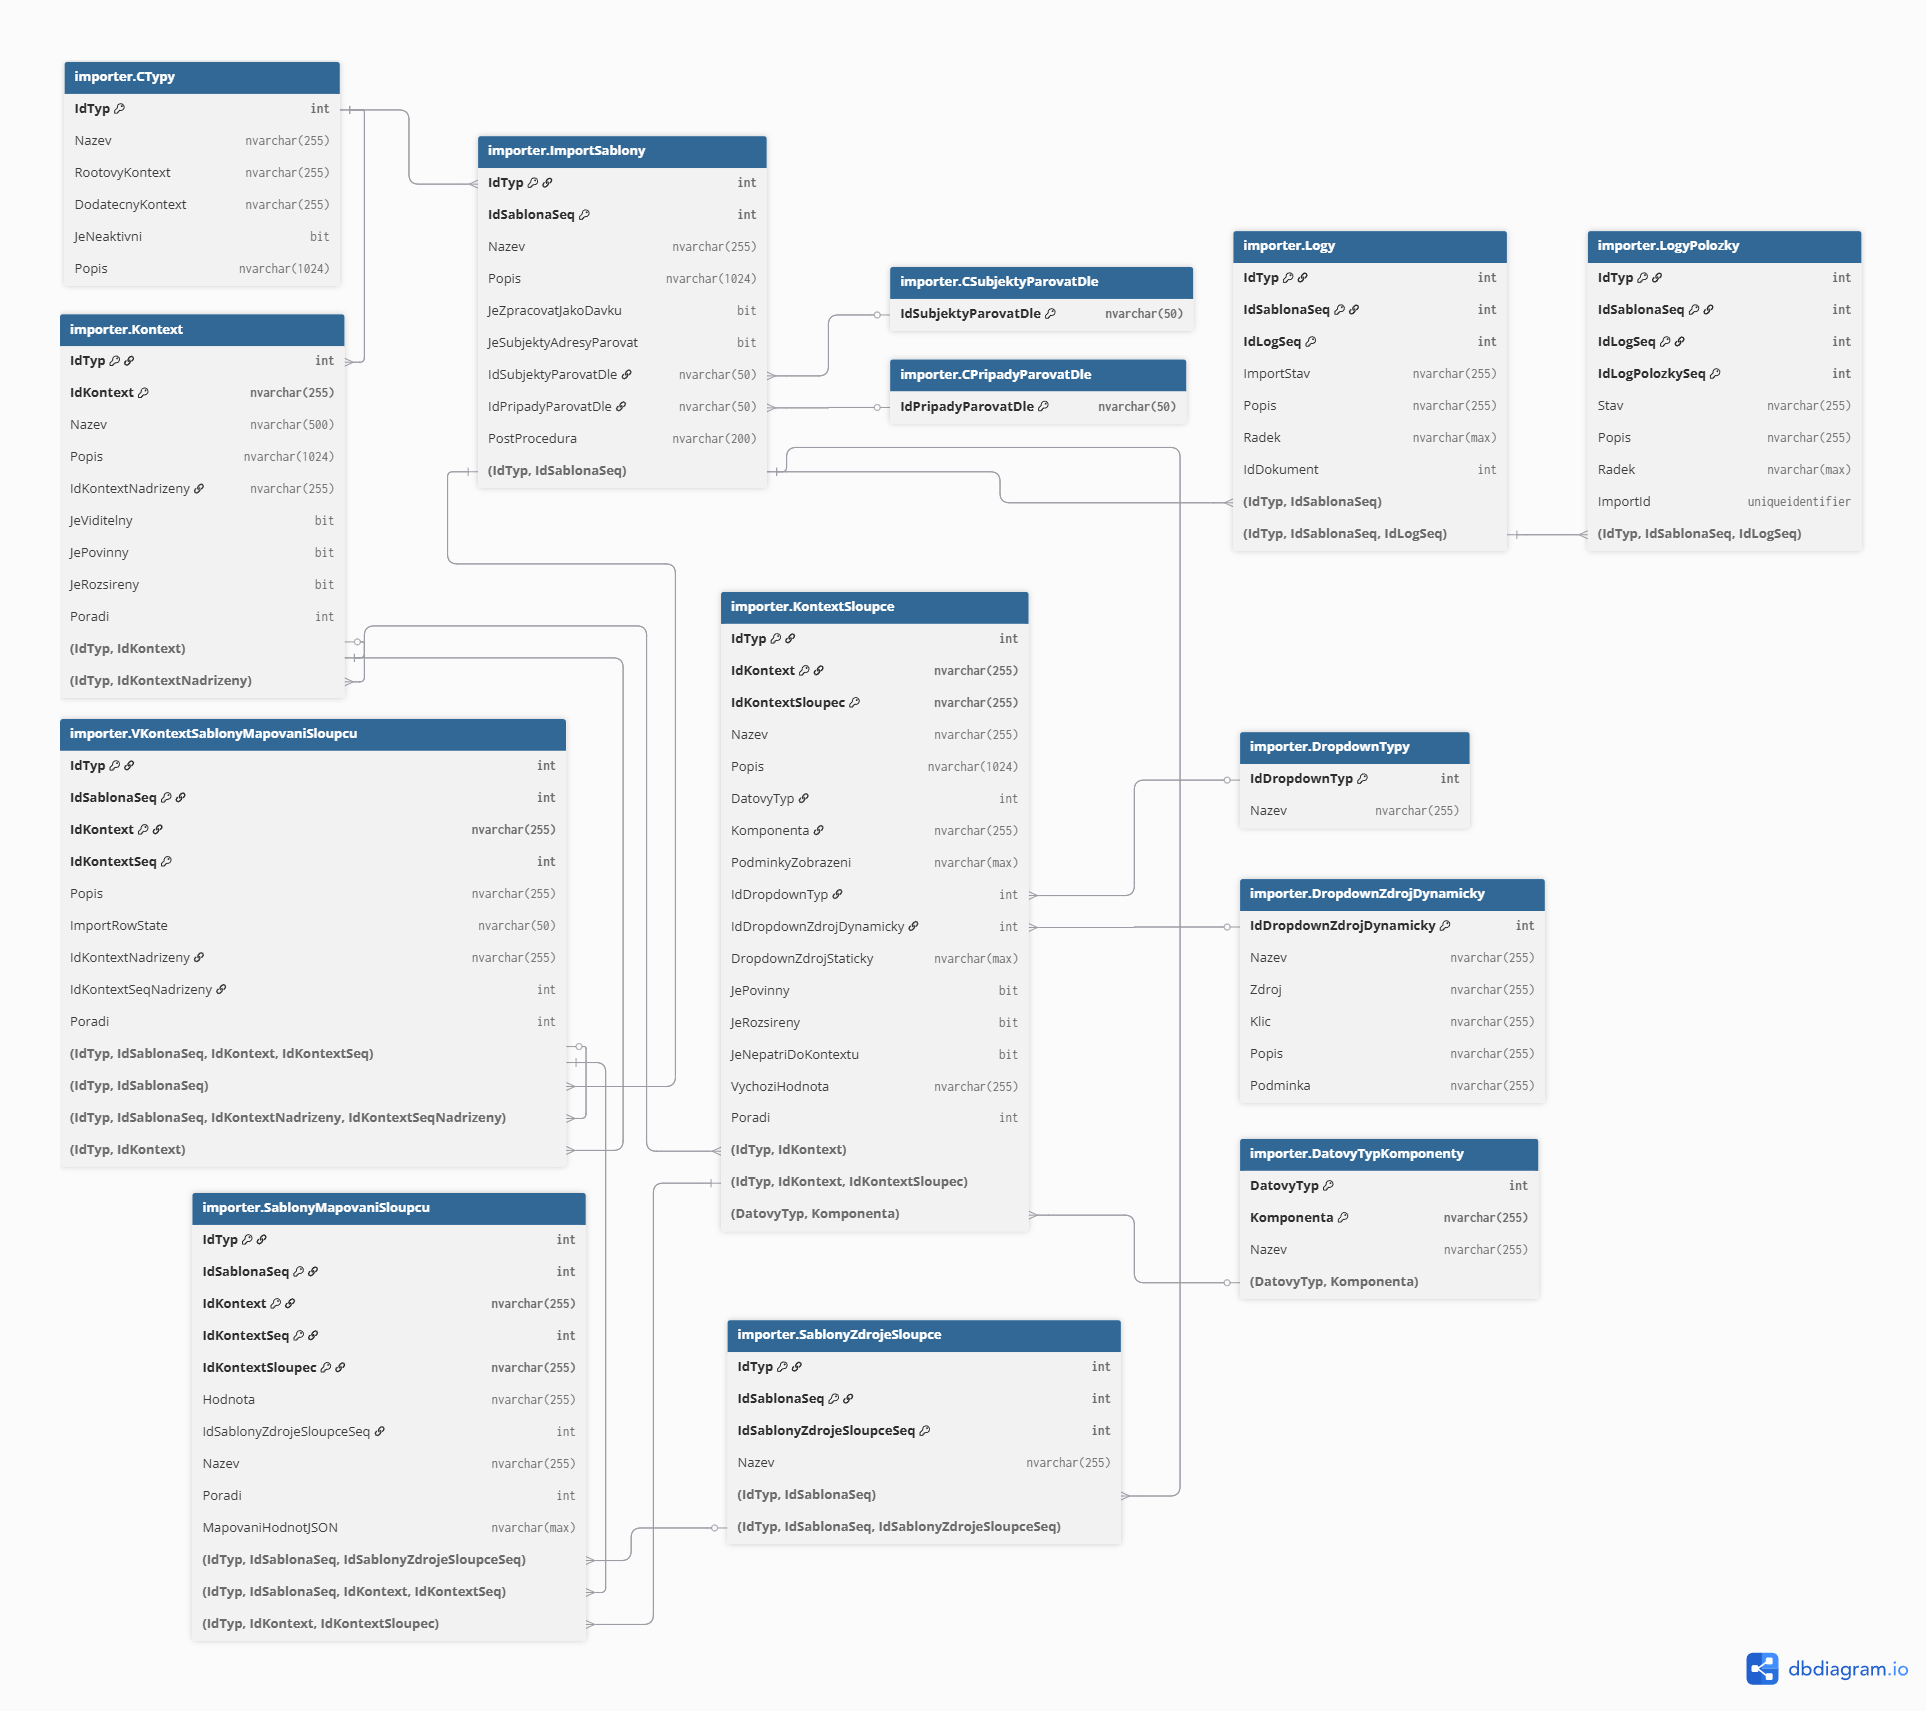
\includegraphics[width=0.8\textwidth]{Figures/ERD_Importer.png}
    \caption{Zjednodušený ER diagram databázového schématu Importer}
    \label{fig:erd_diagram}
\end{figure}

\section{Serverová část a aplikační logika}

Backendová část řešení je implementována v jazyce C\# \cite{csharp_docs} jako \textbf{Service Fabric Actor} v rámci platformy EFabric. Jedná se o mikroslužbu běžící v prostředí Microsoft Azure \cite{microsoft_servicefabric}.

Propojení s jádrem systému zajišťuje třída \texttt{ImporterContext}, která dědí z \texttt{EMapContext}. Samotný proces importu probíhá asynchronně ve dvou fázích: nejprve validace a příprava dat (\texttt{CreateImportAsync}) a následně fyzický zápis do cílových tabulek (\texttt{DirectImportAsync}).

\section{Uživatelské rozhraní (Frontend)}

Prezentační vrstva modulu Importér představuje nejrozsáhlejší část realizace. Je navržena jako autonomní feature modul (\texttt{ImporterModule}) v rámci enterprise architektury systému Evolio, využívající verzi \textbf{Angular 17} \cite{angular_docs} a \textbf{TypeScript} \cite{typescript_docs}.

\subsection{Architektura a hierarchie komponent}

Modul je dekomponován na osm specializovaných komponent, které spolupracují na zajištění plynulého uživatelského zážitku při zpracování dat. Využití komponentového přístupu umožňuje oddělit logiku zobrazení od orchestrace dat. Detailní přehled všech komponent uvádí tabulka \ref{tab:fe_components_full}.



\begin{table}[h]
\centering
\caption{Kompletní přehled komponent modulu Importér}
\label{tab:fe_components_full}
\begin{tabular}{|l|p{9cm}|}
\hline
\textbf{Komponenta} & \textbf{Účel a hlavní funkce} \\ \hline
\texttt{ImporterDetailComponent} & Hlavní dashboard. Zobrazuje typy importů, historii logů a náhled dat ze souboru. \\ \hline
\texttt{ImporterMappingComponent} & Klíčová obrazovka pro definici mapování sloupců Excelu na kontexty systému. \\ \hline
\texttt{ContextTreeComponent} & Rekurzivní komponenta pro vizualizaci a navigaci v hierarchickém stromu kontextů. \\ \hline
\texttt{ImporterDropdownComponent} & Specializovaný výběrový prvek pro intuitivní přiřazování sloupců k atributům. \\ \hline
\texttt{ValueMappingModalComponent} & Dialog pro definici transformací hodnot (např. převod textových stavů na číselné ID). \\ \hline
\texttt{DocumentPickerButtonComponent} & Prvek pro nahrávání souborů s podporou validace přípon a velikosti. \\ \hline
\texttt{ImportProgressDialogComponent} & Sleduje průběh importu po řádcích v reálném čase s vizualizací úspěšnosti. \\ \hline
\texttt{ImportLogDetailComponent} & Detailní prohlížeč výsledků a chybových zpráv z proběhlých importů. \\ \hline
\end{tabular}
\end{table}

\begin{figure}[H]
    \centering
    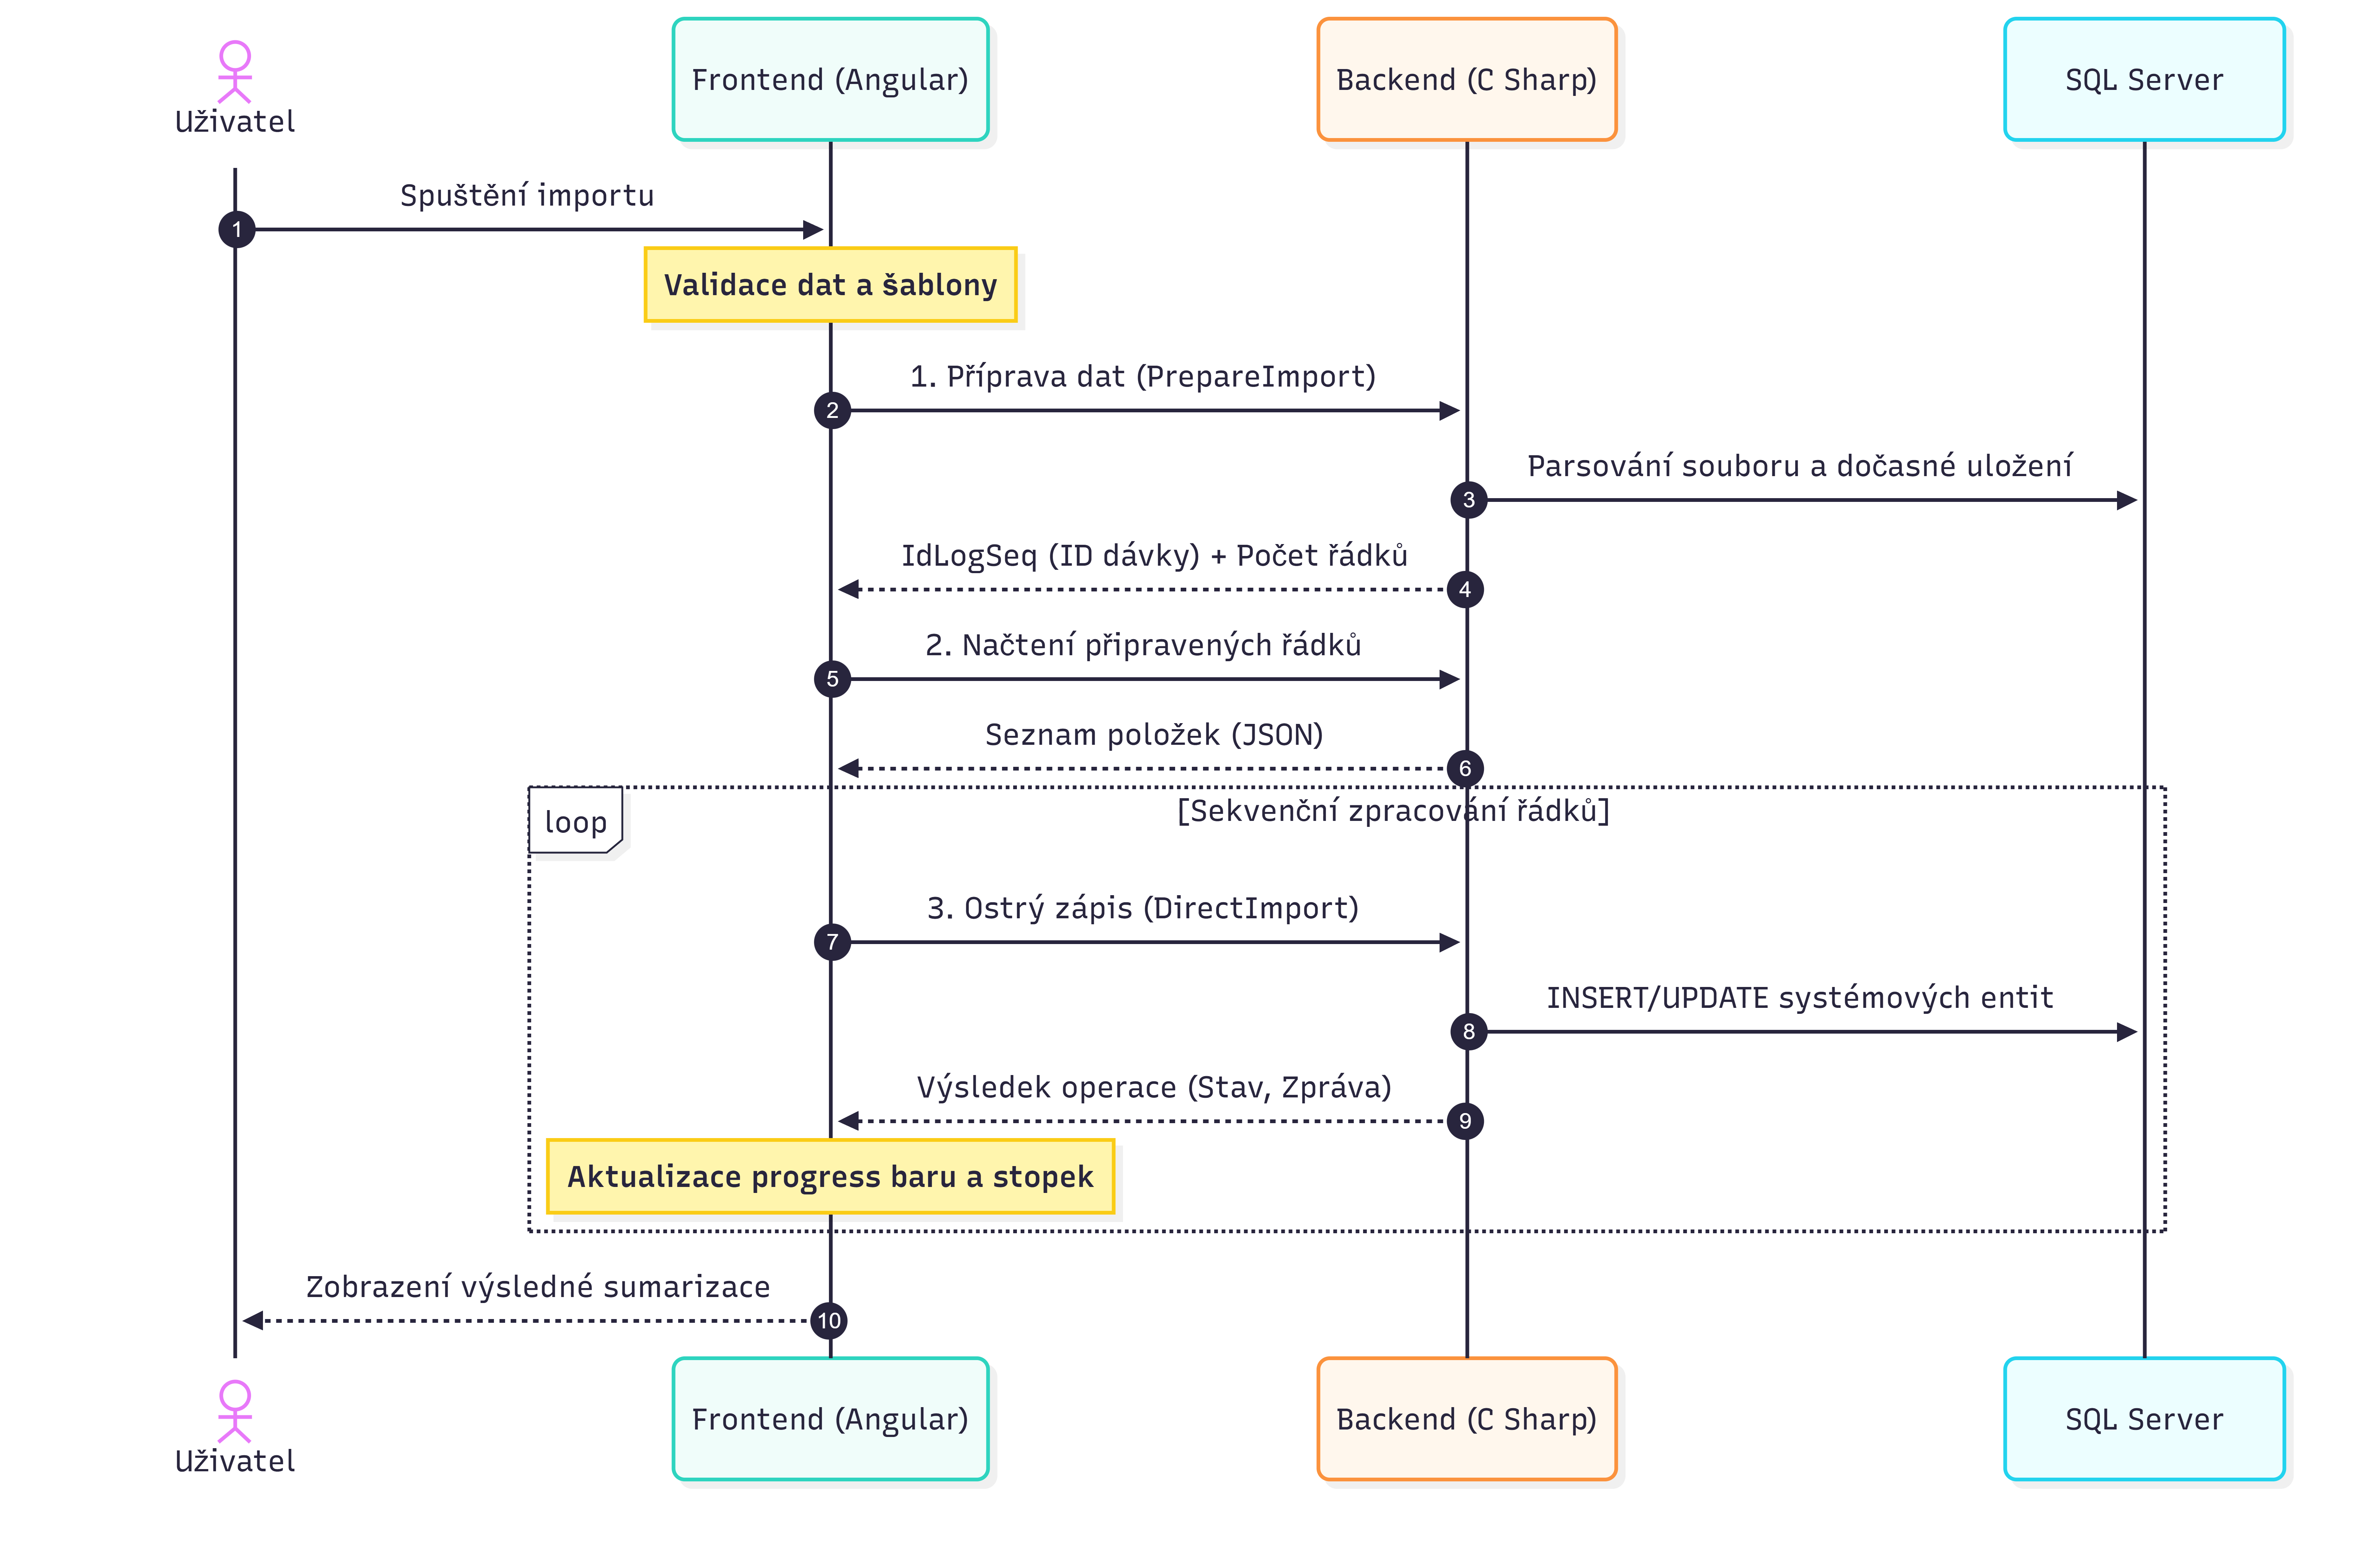
\includegraphics[width=1\textwidth]{Figures/diagram.png}
    \caption{Sekvenční diagram procesu zpracování importu po jednotlivých řádcích}
    \label{fig:import_sequence}
\end{figure}

\subsection{Moderní reaktivní vzory: Signály a RxJS}

Aplikace využívá kombinaci tradiční knihovny RxJS \cite{rxjs_docs} a nového reaktivního primitiva \textbf{Signals}, představeného v Angularu 17. Signály jsou použity pro správu synchronního stavu, který nevyžaduje komplexní transformace, což zjednodušuje kód a zvyšuje čitelnost.

V rámci \texttt{ImporterService} jsou signály využity pro sledování aktuálního kontextu:
\begin{lstlisting}[language=Java, caption={Využití signálů pro správu stavu modulu}]
// Definice signálu pro sledování vybrané šablony
public selectedSablonaId = signal<number | null>(null);

// Výpočetní signál závislý na změně ID
public isSablonaSelected = computed(() => this.selectedSablonaId() !== null);
\end{lstlisting}

Pro asynchronní operace, jako je paralelní načítání číselníků při inicializaci, je nadále využíváno RxJS. Operátor \texttt{forkJoin} zajišťuje, že se aplikace vykreslí až v momentě, kdy jsou k dispozici všechna potřebná metadata:

\begin{lstlisting}[language=Java, caption={Paralelní inicializace dat pomocí forkJoin}]
forkJoin({
  typy: this.emap.get('cTypy', { IdTyp: this.idTyp() }),
  kontexty: this.emap.get('kontext', { IdTyp: this.idTyp() }),
  sablony: this.emap.get('importSablony', { IdTyp: this.idTyp() })
}).pipe(takeUntil(this.destroy$)).subscribe(data => {
  this.state.update(s => ({ ...s, ...data }));
});
\end{lstlisting}

\subsection{Optimalizace výkonu pomocí OnPush strategie}

Z důvodu vysokých nároků na výkon při zobrazování rozsáhlých mapovacích struktur (stromy s desítkami uzlů) byla u všech komponent nasazena strategie \textbf{ChangeDetectionStrategy.OnPush}. 

Tato optimalizace instruuje Angular, aby kontčistých rouroloval změny v komponentě pouze v případě, že se změní její vstupní reference (\texttt{@Input}) nebo je změna explicitně vyžádána. Tím se výrazně redukuje počet cyklů detekce změn při interakci uživatele s formulářem.

\begin{lstlisting}[language=Java, caption={Definice komponenty s OnPush strategií}]
@Component({
  selector: 'ev-importer-mapping',
  templateUrl: './importer-mapping.component.html',
  styleUrls: ['./importer-mapping.component.scss'],
  changeDetection: ChangeDetectionStrategy.OnPush
})
export class ImporterMappingComponent { ... }
\end{lstlisting}

\subsection{Implementace komplexní mapovací logiky}

Jádrem modulu je \texttt{ImporterMappingComponent}, která umožňuje uživateli interaktivně sestavit strukturu importu. Na rozdíl od původního desktopového řešení se zde uplatňuje princip \textit{on-demand} budování struktury:

\begin{itemize}
    \item \textbf{Dynamické instance:} Uživatel může přidávat více instancí stejného kontextu (např. více adres k jednomu subjektu). Každá instance má vlastní stav mapování sloupců.
    \item \textbf{Interaktivní správa:} Stav sbalení a rozbalení jednotlivých sekcí je udržován v \texttt{Set<string>}, což zajišťuje rychlou manipulaci i při velkém počtu prvků.
    \item \textbf{Datová transformace:} Pomocí \textit{pure pipes} dochází k transformaci dat bez nutnosti přepočítávání při každém cyklu detekce změn.
\end{itemize}

\subsection{Real-time monitoring a UX prvky}

Proces importu probíhá sekvenčně, přičemž uživatel je o postupu informován prostřednictvím \texttt{ImportProgressDialogComponent}. Tato komponenta kombinuje několik technologií pro zajištění plynulé zpětné vazby:

\begin{itemize}
    \item \textbf{Sledování času:} Využití knihovny \textit{moment.js} v sekundovém intervalu pro zobrazení doby trvání importu.
    \item \textbf{Inkrementální DataGrid:} Výsledky jsou do tabulky (\textit{DevExtreme DataGrid}) přidávány okamžitě po dokončení požadavku na konkrétní řádek.
    \item \textbf{Vizuální indikátory:} Namísto statických spinnerů jsou v dashboardu využity \textbf{skeleton loadingy}, které predikují strukturu obsahu a snižují kognitivní zátěž uživatele při čekání na data.
\end{itemize}
\chapter{Vývoj AI rozhraní a řešení FE issues}
\label{chap:fe_issues_ai}

Vedle hlavního projektu Importér byla významná část času věnována práci na klientských požadavcích a údržbě existujících systémů. Tato kapitola popisuje vývoj specializovaného AI modulu a řešení specifických chyb v uživatelském rozhraní.

\section{Implementace AI asistenta v prostředí AngularJS}

Jedním z nejnáročnějších úkolů byl vývoj inteligentního chatu pro specifického klienta, jehož informační systém je postaven na starší technologii \textbf{AngularJS (v1.x)} \cite{angularjs_docs}. Cílem bylo integrovat moderní jazykové modely (LLM) do tohoto prostředí a umožnit uživatelům nejen konverzaci, ale i analýzu nahraných dokumentů.

Je důležité podotknout, že framework AngularJS je v současnosti již ve fázi ukončené podpory (\textit{end-of-life}, oficiálně od 31.~12.~2021 \cite{angularjs_eol}) a v rámci standardních firemních procesů jej pro nové projekty již nenasazujeme. Volba této technologie byla v tomto případě čistě pragmatická a vynucená architekturou stávajícího informačního systému klienta. Cílem bylo vyhovět požadavku na integraci moderních funkcí do již zavedené aplikace a zajistit její další rozvoj bez nutnosti okamžité a nákladné migrace celého systému na modernější platformu.

\begin{sidewaysfigure}
    \centering
    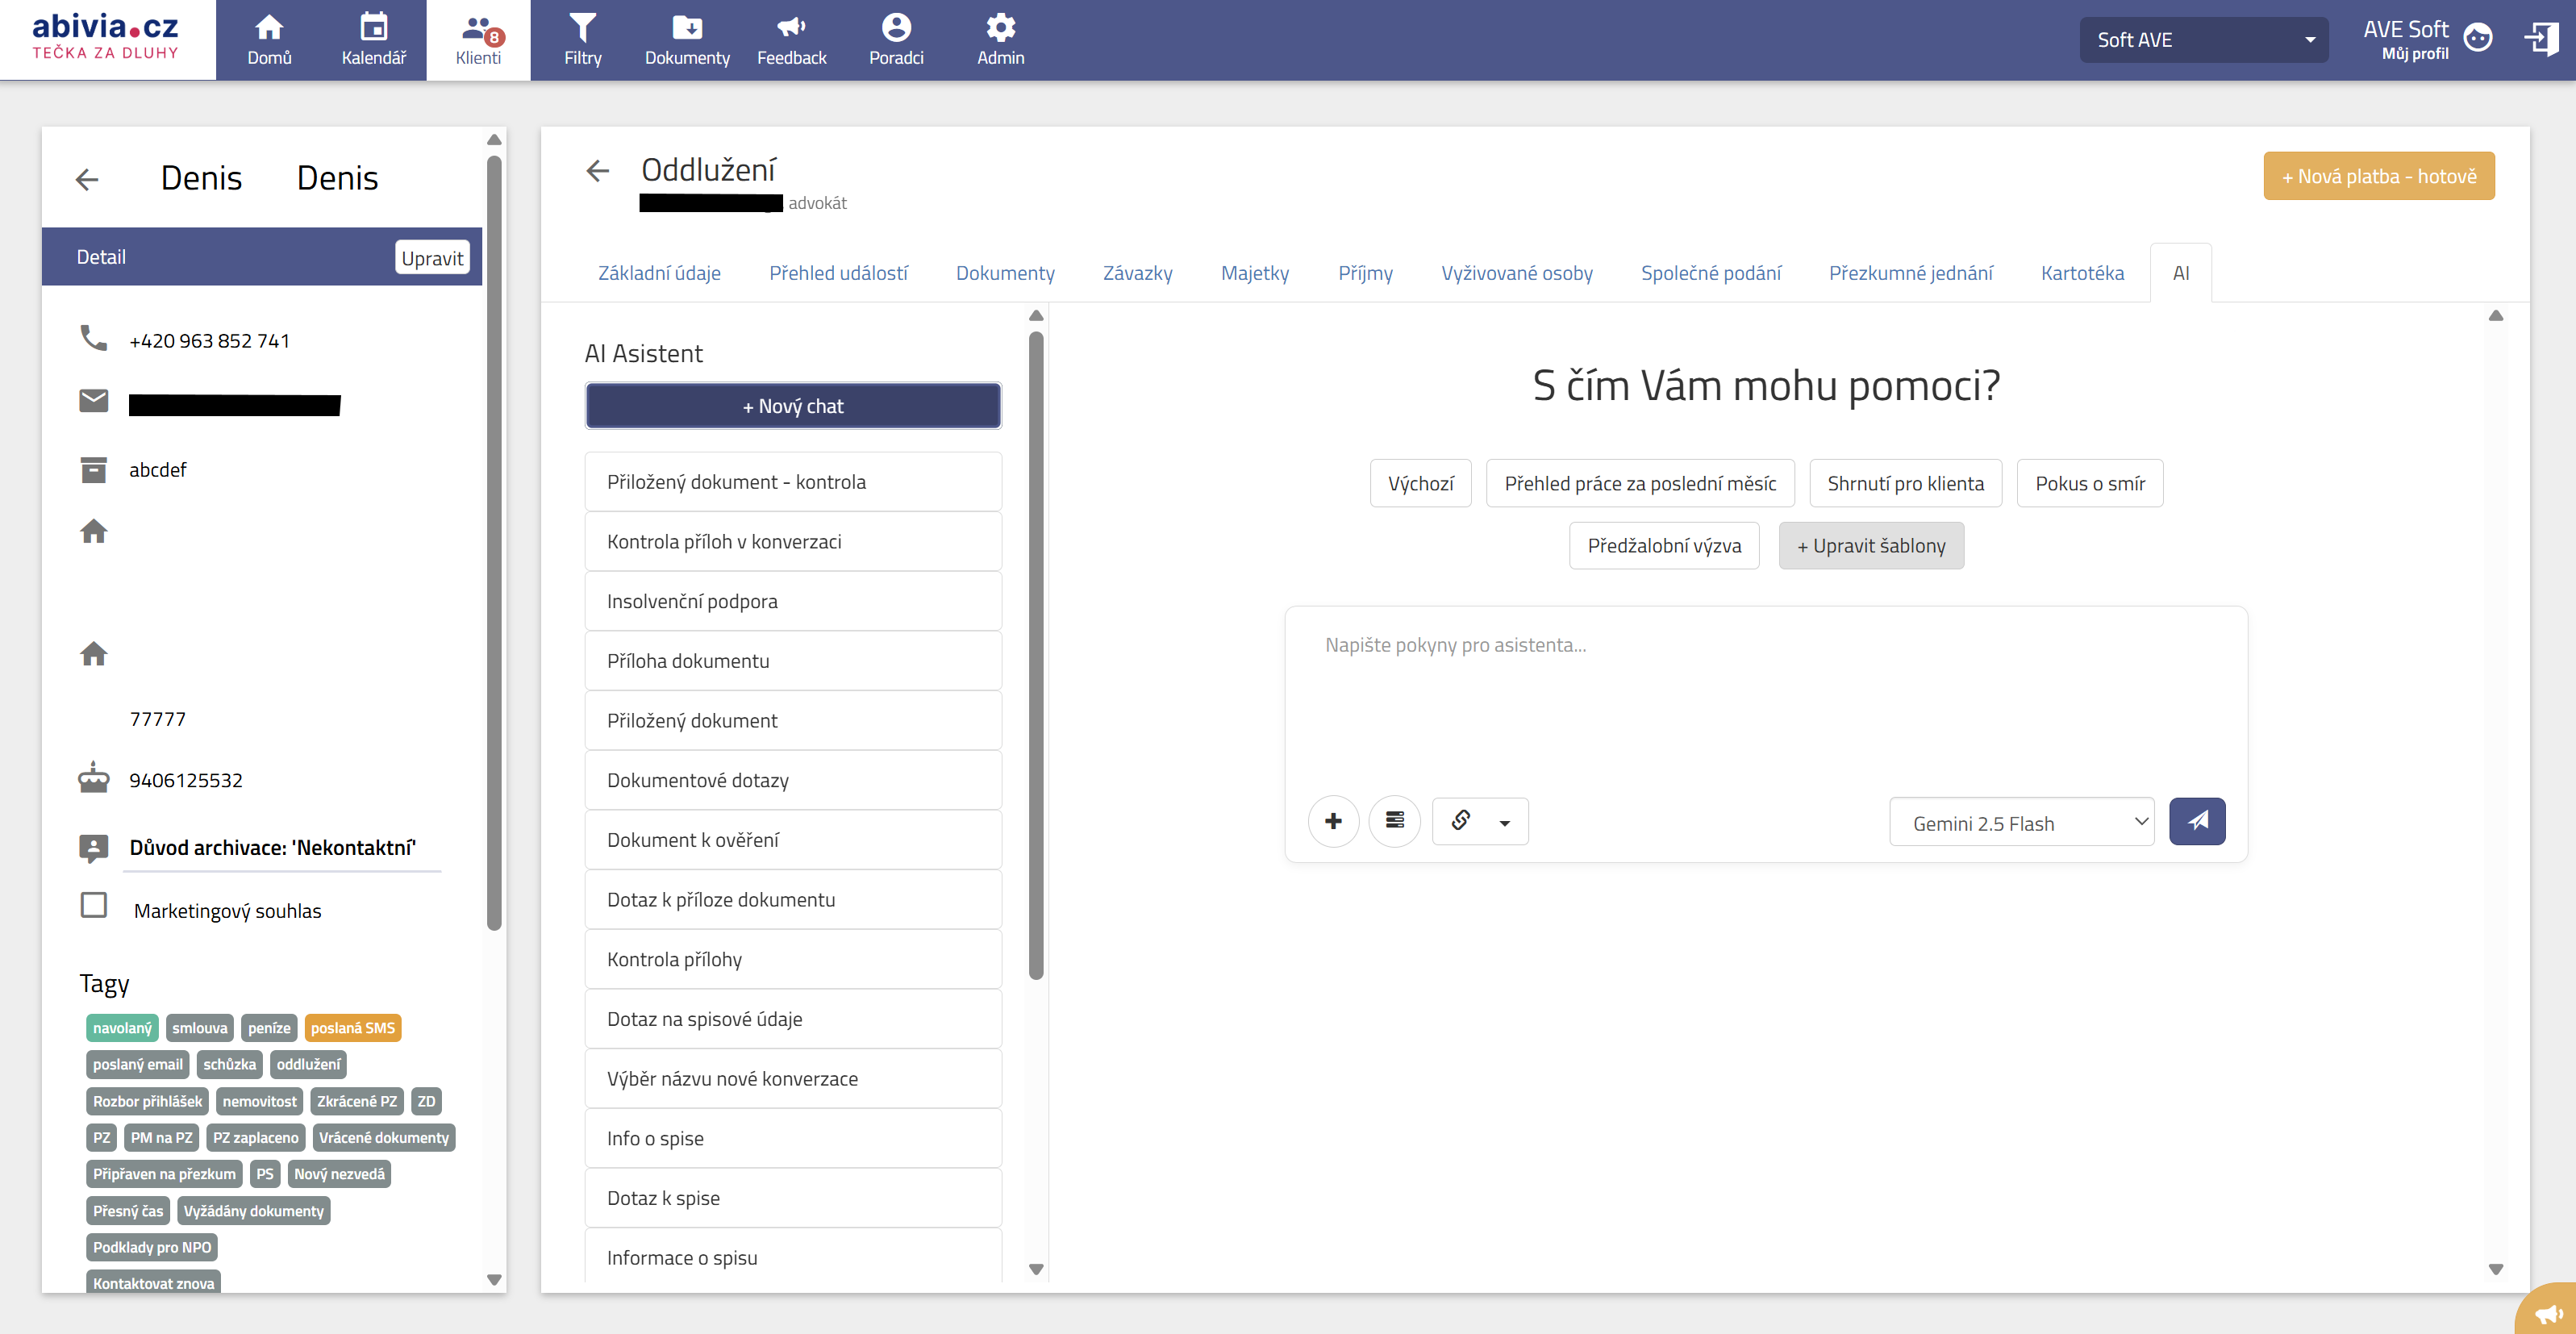
\includegraphics[width=1\textheight]{Figures/AI-new_chat.png}
    \caption{Výchozí rozhraní AI asistenta s nabídkou předdefinovaných šablon (\textit{prompt templates}) a volbou jazykového modelu}
    \label{fig:ai_templates}
\end{sidewaysfigure}

\subsection{Architektura řešení a datový tok}

Modul je rozdělen do tří vrstev, které společně zajišťují celý životní cyklus konverzace -- od odeslání dotazu až po streamování odpovědi zpět do uživatelského rozhraní. Jejich zodpovědnosti shrnuje tabulka \ref{tab:ai_layers}.

\begin{table}[H]
\centering
\caption{Vrstvy AI modulu a jejich zodpovědnosti}
\label{tab:ai_layers}
\begin{tabular}{|l|p{9cm}|}
\hline
\textbf{Vrstva} & \textbf{Zodpovědnost} \\ \hline
Prezentační (AngularJS) & Správa vláken (\textit{threads}) konverzace, rendering Markdown výstupu, upload dokumentů, sběr tokenů streamu. \\ \hline
Aplikační (C\# Service Fabric) & Orchestrace: příjem dotazu, konstrukce promptu, volání LLM API, publikace tokenů do SignalR hubu. \\ \hline
Externí LLM API & Generování odpovědi (Azure OpenAI / OpenAI \cite{openai_api}); streaming tokenů přes rozhraní Chat Completions. \\ \hline
\end{tabular}
\end{table}

Vzhledem k požadavku na plynulé zobrazování odpovědi (podobně jako v chatovacích rozhraních typu ChatGPT) nebylo možné čekat na vygenerování celé odpovědi na serveru. Řešení využívá technologii \textbf{SignalR} \cite{signalr_docs} pro real-time přenos jednotlivých tokenů textu v momentě jejich vygenerování.

Datový tok od okamžiku odeslání dotazu je následující:
\begin{enumerate}
    \item Frontend odešle HTTP POST požadavek s dotazem, identifikátorem vlákna (\texttt{partitionKey}, \texttt{rowKey}) a identifikátorem vybraného modelu (\texttt{selectedModelId}).
    \item Backendová služba \texttt{AiAgents\_Threads} dohledá konverzační vlákno v úložišti, načte jeho historii a sestaví kompletní prompt pro LLM (systémový prompt + historie zpráv + aktuální dotaz).
    \item Backend iniciuje volání Chat Completions API s parametrem \texttt{stream = true}; přijaté SSE události postupně publikuje přes SignalR hub zpět na klienta.
    \item Frontend je přihlášen k odběru události \texttt{openAIStream}; každý příchozí fragment (chunk) inkrementálně připojuje k aktuální zprávě a vynucuje překreslení UI.
    \item Po ukončení streamu backend pošle řídicí zprávu \texttt{refreshStatus = REFRESH}, která klienta informuje o dokončení a zároveň uvolní blokaci odesílacího tlačítka.
\end{enumerate}

\begin{lstlisting}[language=JavaScript, caption={Zpracování streamované odpovědi v AngularJS}]
// Naslouchání na notifikace ze SignalR hubu
hub.on('openAIStream', function(message) {
    $rootScope.$broadcast('openAIStream', message);
});

// Skládání zprávy v kontroleru (ev. zdroj: contractDetail.ts)
$scope.$on('openAIStream', function(event, chunk) {
    // Inkrementální připojení tokenu k aktuální streamované zprávě
    streamingMsg.Message += chunk;
    // Vynucení digest cyklu mimo Angular kontext
    $scope.$applyAsync();
});

// Ukončení streamu a uvolnění UI
$scope.$on('refreshStatus', function(event, status) {
    if (status === 'REFRESH') {
        $scope.isStreaming = false;
        $scope.isLoading = false;
    }
});
\end{lstlisting}

\subsection{Správa vláken konverzace a historie}

Každá konverzace je v systému reprezentována samostatným \textbf{vláknem} (\textit{thread}) identifikovaným dvojicí \texttt{partitionKey} a \texttt{rowKey} (klíče úložiště Azure Table Storage v rámci Service Fabric služby). Vlákno uchovává:
\begin{itemize}
    \item seznam všech zpráv (role \texttt{user} / \texttt{assistant}) v chronologickém pořadí,
    \item identifikátor zvoleného modelu (\texttt{idaiModel}), který je závazný pro celé vlákno,
    \item seznam vazeb na nahrané dokumenty (dokumenty se ukládají odděleně a do vlákna se připojují pouze reference).
\end{itemize}

Takto oddělené úložiště umožňuje efektivně iterovat nad historií bez nutnosti přenášet celé dokumenty, a zároveň poskytuje klientovi seznam vláken k výběru (boční panel konverzací).

Při odesílání nové zprávy frontend prostřednictvím metody \texttt{createThread()} buď pokračuje v existujícím vláknu, nebo jej nově zakládá. Výběr modelu je při prvním založení vlákna iniciálně nastaven na model označený v databázi jako výchozí (\texttt{jeVychozi = true}); uživatel jej může přepnout při vytváření vlákna, po zahájení konverzace je však model uzamčen pro zajištění konzistence odpovědí v rámci téhož vlákna.

\subsection{Zpracování nahraných dokumentů}

Klíčovým požadavkem byla analýza právních dokumentů. Tato funkce vyžadovala specifický dvoufázový proces:

\paragraph{Fáze 1 -- Upload.} Po výběru dokumentů uživatelem jsou soubory odeslány na endpoint \texttt{AiAgents\_Docs\_Upload\_ById} voláním \texttt{\$q.all()} pro paralelní zpracování. Backend každý dokument extrahuje do textové podoby (pro PDF, DOCX a obdobné formáty), uloží do trvalého úložiště a vrátí identifikátor \texttt{idDokument}. Během uploadu je UI blokováno (\texttt{uploadInProgress = true}) a odesílací tlačítko je deaktivováno.

\paragraph{Fáze 2 -- Vazba na zprávu.} Po dokončení uploadu všech souborů frontend přidá do aktuální zprávy kolekci referencí (\texttt{idDokument}, název souboru, přípona) a teprve poté zahájí samotné volání \texttt{createThread()}. Backend při sestavování promptu pro LLM načte extrahovaný obsah referencovaných dokumentů a zařadí jej do kontextového okna jazykového modelu. Tento přístup (označovaný jako \textit{in-context document loading}) je jednodušší alternativou ke vzoru Retrieval-Augmented Generation (RAG) a je vhodný pro scénáře, kde je celý dokument dostatečně malý, aby se vešel do kontextového okna modelu.

\subsection{Formátování výstupu a Markdown rendering}

Jazykové modely generují odpověď ve formátu Markdown. Pro korektní zobrazení byla nasazena knihovna \textbf{marked.js}, která v reálném čase konvertuje text na HTML. Konfigurace potlačila automatické generování ID nadpisů a mangling e-mailových adres:

\begin{lstlisting}[language=JavaScript, caption={Konfigurace Markdown parseru (marked.js)}]
const markedInstance = window.marked;
if (markedInstance && typeof markedInstance.setOptions === 'function') {
    markedInstance.setOptions({ mangle: false, headerIds: false });
}
\end{lstlisting}

Protože je rendering volán při každém tokenu, bylo nutné ošetřit i částečně dokončené bloky (např. neukončený \texttt{```} blok kódu); při nekonzistentním stavu zůstává text v surové podobě až do doručení dalšího fragmentu.

\subsection{Ošetření chybových stavů}

Streamované API přináší specifické chybové stavy, které klasické REST volání neřeší:
\begin{itemize}
    \item \textbf{Přerušení streamu na backendu} -- backend publikuje událost \texttt{openAIError}, klient uvolní UI a zobrazí informaci o selhání.
    \item \textbf{Selhání uploadu dokumentu} -- při selhání kteréhokoliv souboru je \texttt{\$q.all()} odmítnut, UI odstraní přidané zprávy a konverzace se vrátí do výchozího stavu.
    \item \textbf{Ztráta SignalR spojení} -- klient volá \texttt{signalRService.connect(contextGuid)}, který při výpadku automaticky navazuje reconnect.
\end{itemize}

\clearpage
\begin{sidewaysfigure}
    \centering
    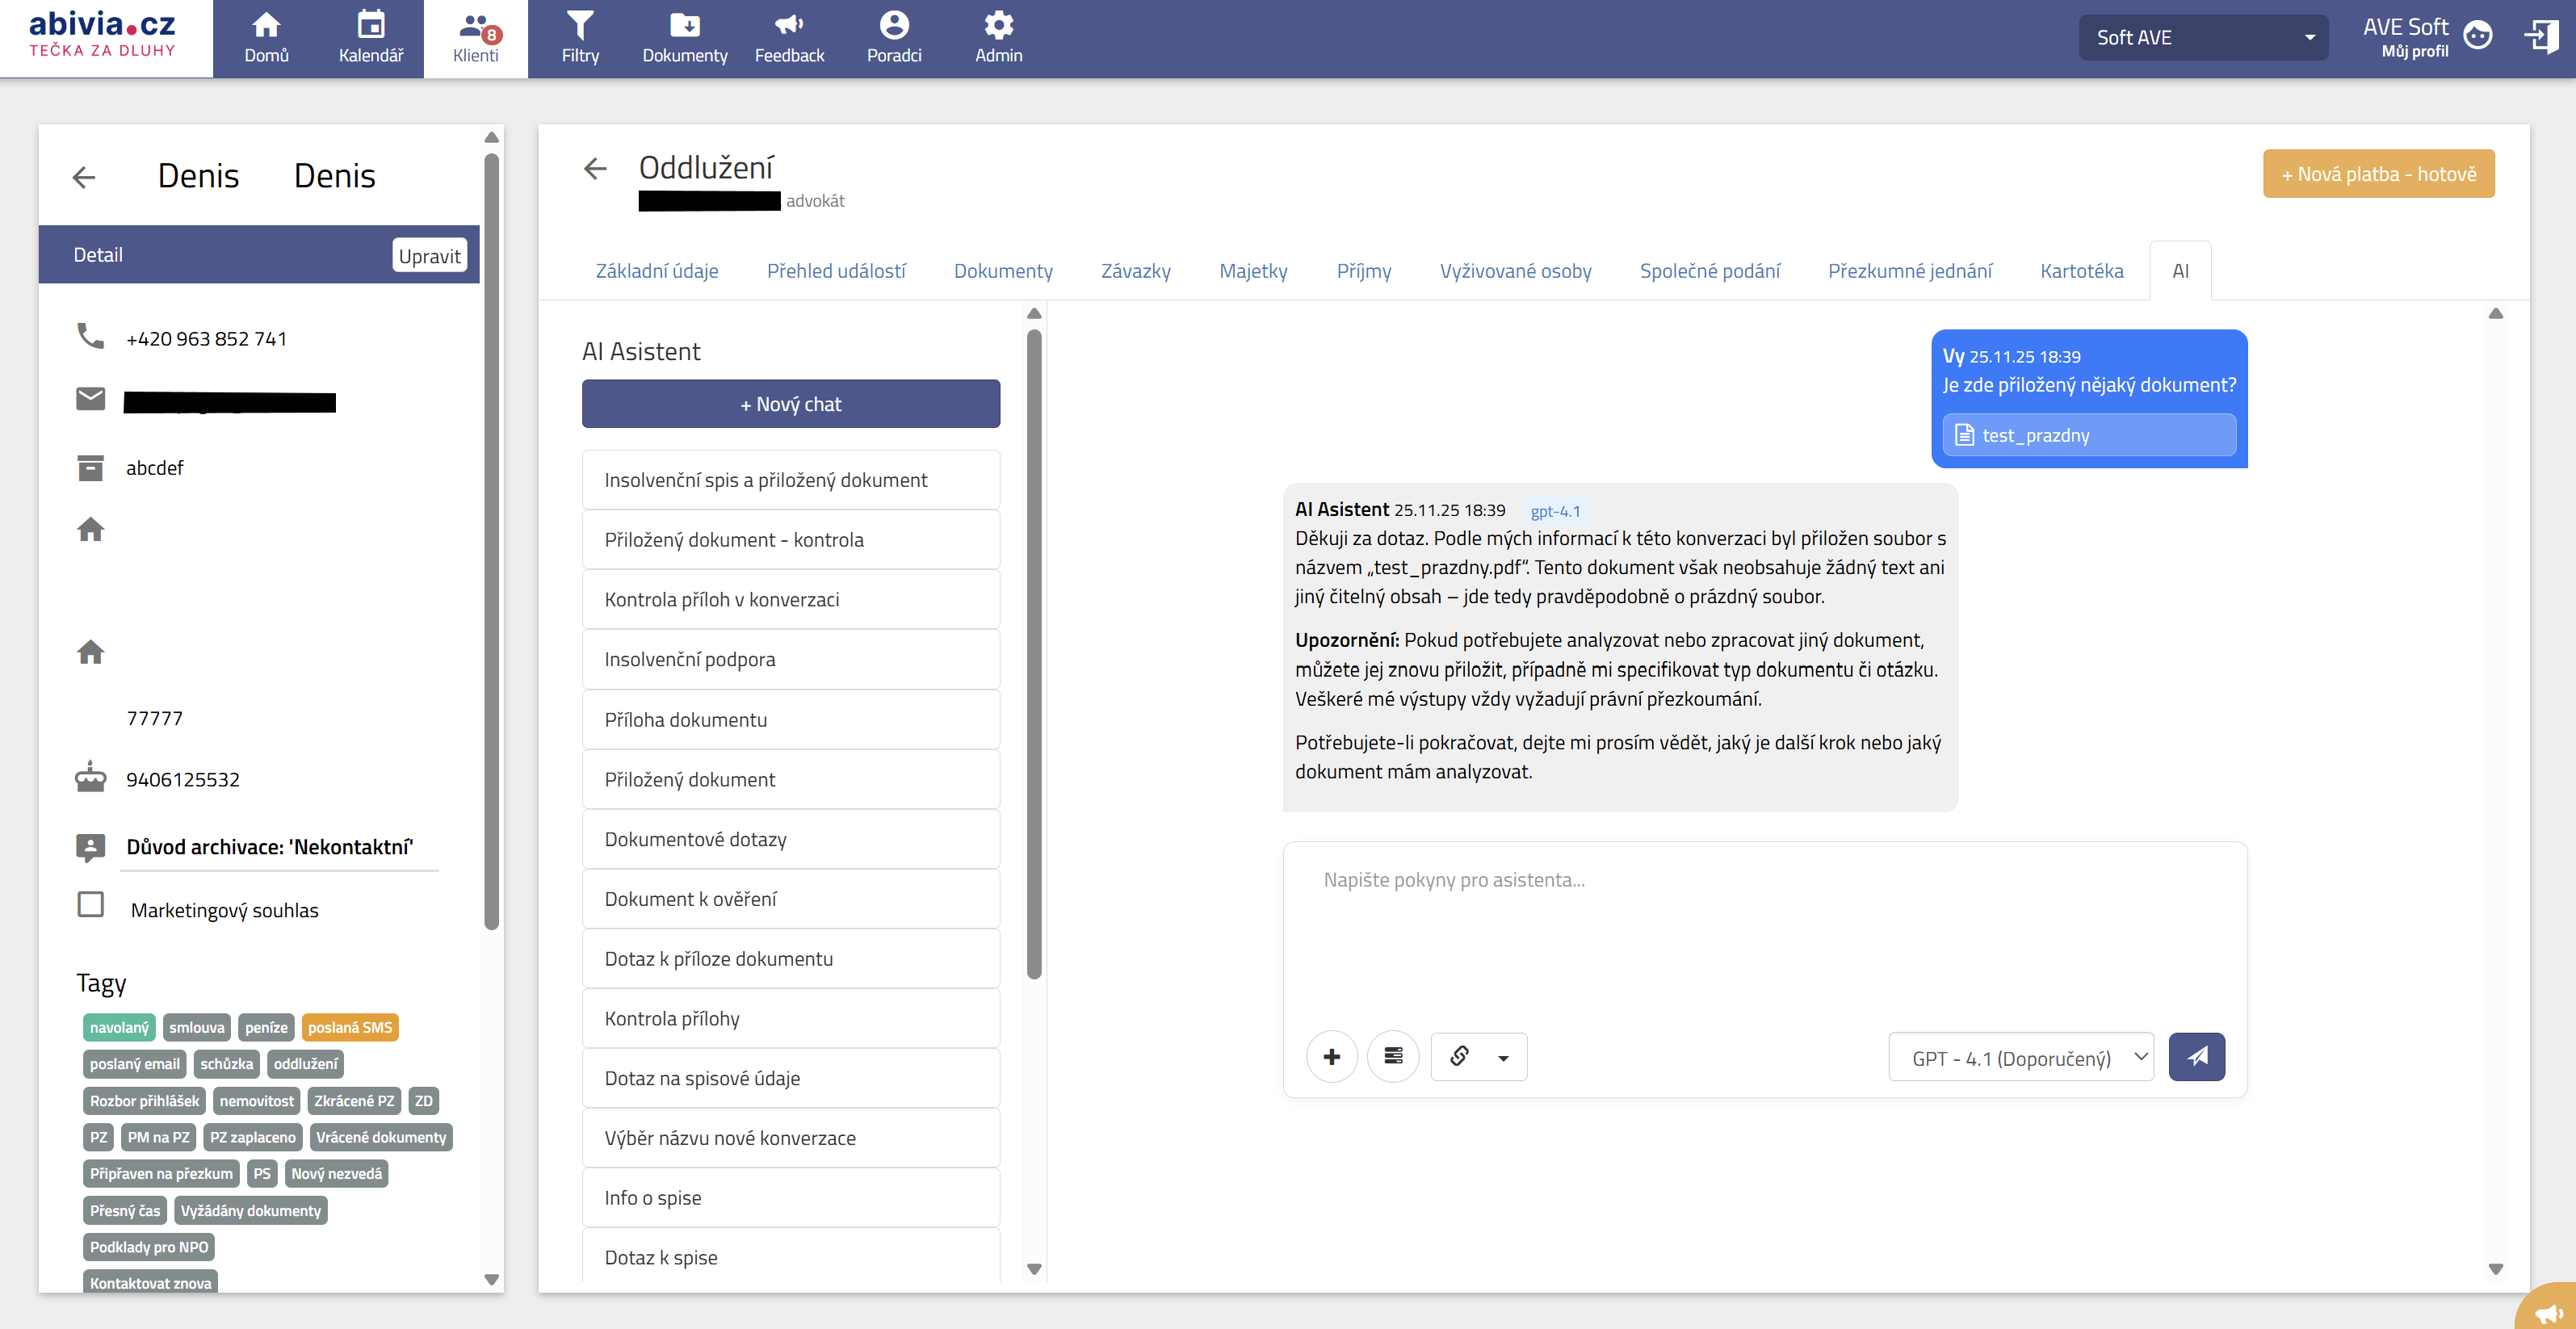
\includegraphics[width=1\textwidth]{Figures/AI-existing_chat.png}
    \caption{Ukázka probíhající konverzace s formátováním textu (Markdown) a analýzou nahraného dokumentu}
    \label{fig:ai_conversation}
\end{sidewaysfigure}
\clearpage


\section{Řešení chyb v uživatelském rozhraní (opravy chyb)}

Nedílnou součástí praxe byla analýza a opravy chyb v systému Evolio. Příkladem komplexního problému byla chyba v komponentě Přehledy (založené na knihovně DevExpress \cite{devexpress_docs}), kde docházelo k selhání načítání filtrů.

\subsection{Analýza problému: Konflikt seskupování a ukotvení}
Uživatelé hlásili, že u určitých přehledů se nenačetla data v tabulce a došlo k permanentnímu stavu načítání (spinner se nezastavil). Analýzou bylo zjištěno, že problém nastává v momentě, kdy je sloupec nastaven jako \textbf{ukotvený} (Fixed) a zároveň se podle něj \textbf{seskupuje} (Grouped).

Komponenta DevExpress v této specifické konfiguraci nedokázala správně vypočítat pozici elementů, což vedlo k chybě v konzoli a k tomu, že se data tabulky nenačetla.

\begin{figure}[H]
    \centering
    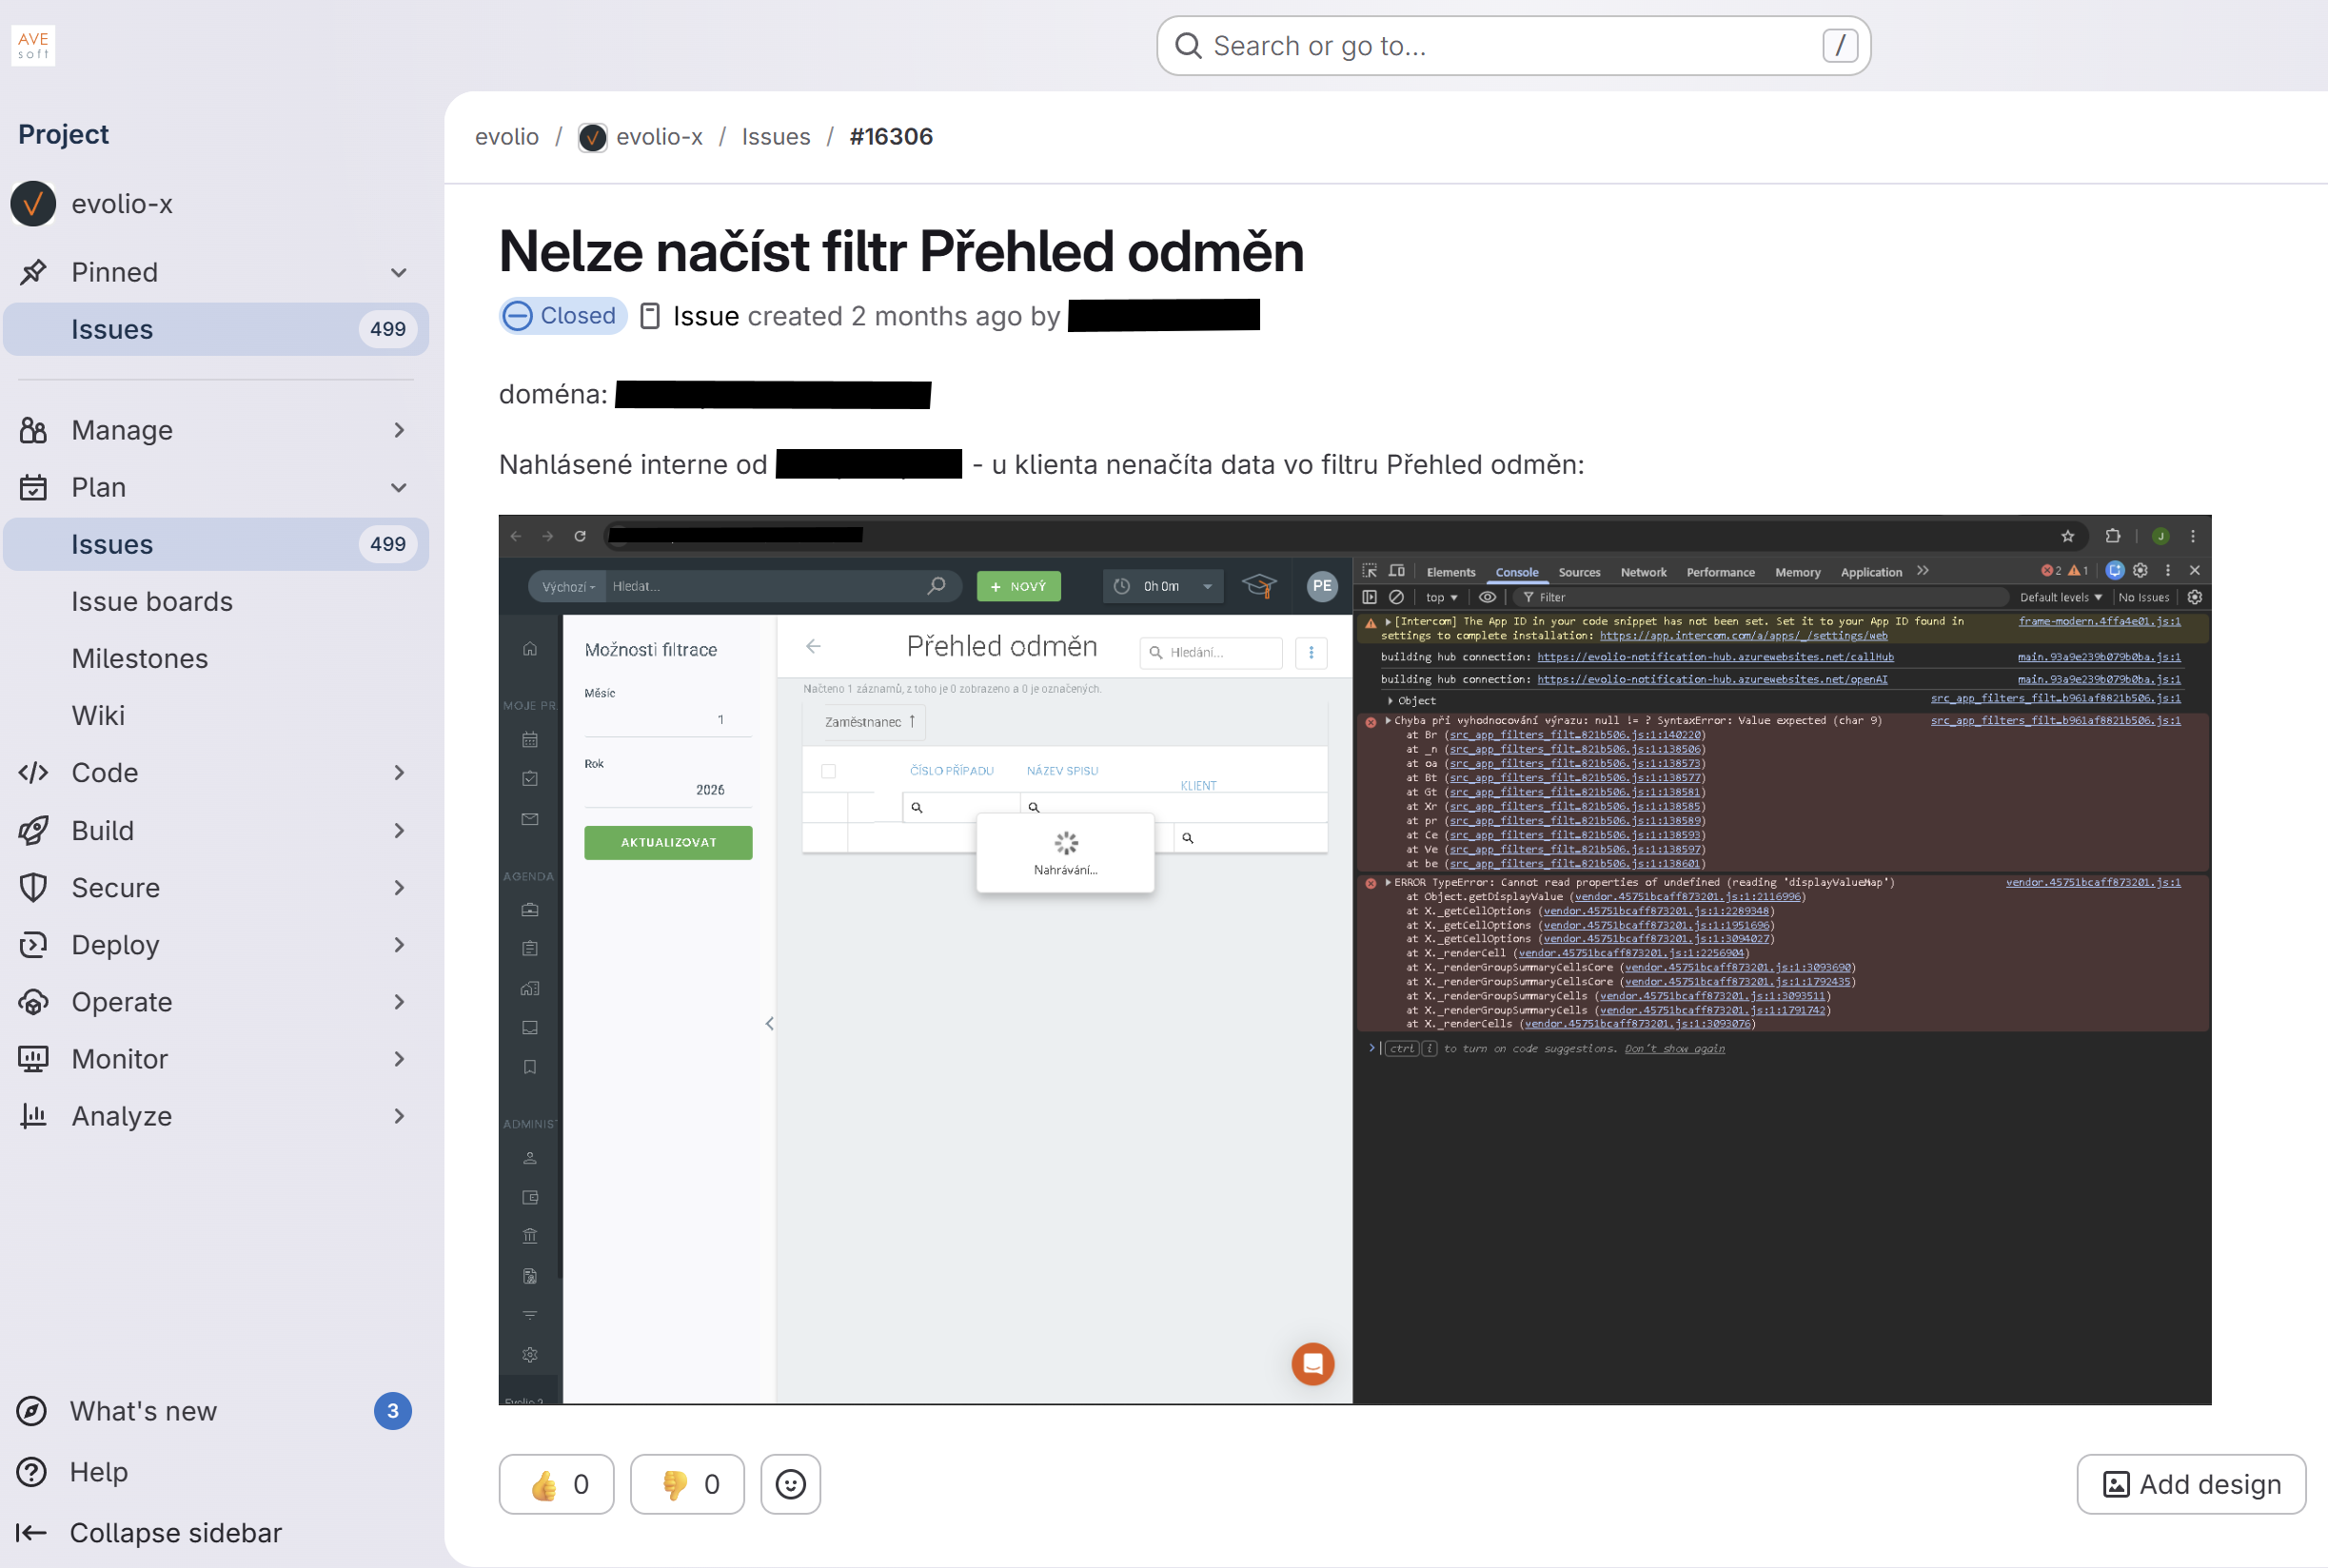
\includegraphics[width=1\textwidth]{Figures/gitlab-issue.png}
    \caption{Ukázka zadaného požadavku (issue) v systému GitLab popisující nekonzistentní chování tabulky při kombinaci Fixed + Grouped}
    \label{fig:gitlab-issue}
\end{figure}

\subsection{Implementace opravy}
Oprava spočívala v úpravě logiky, která generuje konfiguraci pro sloupce tabulky. Bylo nutné zajistit, aby se vlastnost \texttt{fixed} automaticky deaktivovala, pokud je sloupec použit pro seskupování.

\begin{lstlisting}[language=JavaScript, caption={Úprava konfigurace sloupců pro detekci konfliktu Fixed/Grouped}]
// Puvodni problematicky kod
// fixedPosition: colcf.fixed !== null ? colcf.fixed.toLowerCase() : null,
// fixed: colcf.fixed !== null,

// Nova logika s osetrenim konfliktu
const isFixed = colcf.fixed !== null &&
                colcf.fixed.toLowerCase() !== 'none' &&
                !colcf.grouped; // Klicova podminka: nesmi byt seskupeno

// Aplikace do konfigurace
const columnConfig = {
    // ... ostatni vlastnosti
    fixedPosition: isFixed ? colcf.fixed.toLowerCase() : null,
    fixed: isFixed
};
\end{lstlisting}

Tato úprava zajistila stabilitu komponenty i v případě, že uživatel (nebo uložený přehled) definoval tuto konfliktní kombinaci vlastností.

\chapter{Automatizované testování}
\label{chap:testing}

Pro zajištění kvality a stability systému Evolio existuje v rámci firemní infrastruktury sada automatizovaných UI testů. Tyto testy simulují reálné chování uživatele v prohlížeči a slouží jako regresní testování po nasazení nové verze aplikace. V rámci praxe jsem se do tohoto projektu zapojil -- rozšiřoval jsem stávající sadu o nové testovací scénáře a průběžně pečoval o funkčnost již existujících testů.

\section{Metodika a zařazení v testovací pyramidě}

Automatizované testování softwaru bývá zpravidla strukturováno podle tzv. \textit{testovací pyramidy} \cite{fowler_test_pyramid, meszaros_xunit}, která rozlišuje tři vrstvy testů podle granularity a rychlosti zpětné vazby:

\begin{table}[H]
\centering
\caption{Vrstvy testovací pyramidy a jejich pokrytí v projektu Evolio}
\label{tab:test_pyramid}
\begin{tabular}{|l|p{4cm}|p{3.5cm}|p{3.5cm}|}
\hline
\textbf{Vrstva} & \textbf{Účel} & \textbf{Nástroje v Evoliu} & \textbf{Moje zapojení} \\ \hline
Unit testy & Izolované testování jednotek kódu (metody, třídy). & NUnit, Moq (v dílčích modulech). & Minimální -- moduly, na kterých jsem pracoval, mají nízké pokrytí unit testy. \\ \hline
Integrační testy & Ověření spolupráce více komponent (služba + DB). & Vlastní framework nad .NET + testovací SQL instance. & Žádné -- nebyly předmětem praxe. \\ \hline
UI / E2E testy & Simulace uživatele v prohlížeči; validace end-to-end scénářů. & Selenium WebDriver, NUnit, Boa.Constrictor. & Hlavní oblast praxe -- rozšiřování a údržba. \\ \hline
\end{tabular}
\end{table}

UI testy stojí na vrcholu pyramidy; jsou nejpomalejší a nejnáchylnější k nestabilitě (tzv. \textit{flaky tests}), ale zároveň poskytují nejbližší aproximaci reálného uživatelského scénáře. Jejich hodnota spočívá v tom, že odhalí chyby vznikající na rozhraní mezi vrstvami -- například selhání komunikace mezi frontendem a backendem nebo chybně vyrenderované UI prvky, které unit test nemůže odhalit.

\section{Strategie a nástroje}

Jako technologický základ byl zvolen framework \textbf{Selenium WebDriver} \cite{selenium_docs}, který je v .NET prostředí de facto standardem pro automatizaci webových prohlížečů. Pro samotné spouštění testů a validaci podmínek (assertions) je využit framework \textbf{NUnit} \cite{nunit_docs} (atributy \texttt{[Test]}, \texttt{[SetUp]}, \texttt{[TearDown]}).

\subsection{Volba návrhového vzoru: Screenplay místo Page Object Modelu}

Pro organizaci testovacího kódu existují dva převládající návrhové vzory. Jejich srovnání shrnuje tabulka \ref{tab:pom_vs_screenplay}.

\begin{table}[H]
\centering
\caption{Porovnání Page Object Model a Screenplay Pattern}
\label{tab:pom_vs_screenplay}
\begin{tabular}{|l|p{5cm}|p{5cm}|}
\hline
\textbf{Aspekt} & \textbf{Page Object Model (POM)} & \textbf{Screenplay Pattern} \\ \hline
Hlavní abstrakce & Stránka (třída reprezentující jednu obrazovku). & Herec (Actor) a jeho akce. \\ \hline
Organizace kódu & Metody jsou vázány na stránku. & Akce jsou samostatné, znovupoužitelné. \\ \hline
Čitelnost testu & Procedurální styl. & Deklarativní, čitelný jako přirozený jazyk. \\ \hline
Škálovatelnost & Při růstu se objevují „God Object" třídy. & Lepší kompozice; nové akce bez zásahu do stránek. \\ \hline
Křivka učení & Nízká. & Vyšší -- vyžaduje pochopení SOLID principů. \\ \hline
\end{tabular}
\end{table}

Projekt UI testů v Evoliu využívá \textbf{Screenplay Pattern} \cite{knight_screenplay} implementovaný pomocí knihovny \textbf{Boa.Constrictor} \cite{boa_constrictor}. Tento přístup se zaměřuje na to, \emph{co} uživatel (Actor) dělá, spíše než na strukturu stránek, a odpovídá principům SOLID -- zejména Single Responsibility Principle, neboť každá akce má jediný důvod ke změně \cite{martin_clean_architecture}.

Základní stavební kameny architektury jsou:
\begin{itemize}
    \item \textbf{Actor (Tester):} Entita provádějící test. V našem případě je instanciována v \texttt{BaseTest} třídě.
    \item \textbf{Task:} Složitější úloha skládající se z více kroků (např. \texttt{Login.WithSessionCredentials()}).
    \item \textbf{Interaction:} Atomická akce (např. \texttt{Click.On(...)}, \texttt{SendKeys.To(...)}).
    \item \textbf{Question:} Dotaz na stav aplikace (např. \texttt{Appearance.Of(...)}, \texttt{ValueAttribute.Of(...)}).
\end{itemize}

\section{Implementace testovacích scénářů}

Testy jsou organizovány do logických celků podle agend (Podatelna, Případy, Subjekty). Následující ukázka demonstruje strukturu CRUD testu pro vytvoření nového subjektu.

\subsection{Příklad: Vytvoření subjektu}
Testovací metoda dodržuje princip \textbf{Arrange-Act-Assert} \cite{beck_tdd}. Využívá fluent syntaxi, která činí test čitelným téměř jako přirozený jazyk.

\begin{lstlisting}[language={[Sharp]C}, caption={Ukázka testu vytvoření subjektu pomocí Screenplay patternu}]
[Test]
public void CreateSubject_Manually_ShouldSucceed()
{
    // Arrange: Priprava dat
    string name = "Testovaci Subjekt " + Guid.NewGuid();
    string ico = "12345678";

    // Act: Provedeni akci (Navigace -> Vyplneni formulare -> Ulozeni)
    Tester.AttemptsTo(Navigate.ToUrl(SubjectPage.Url));
    Tester.AttemptsTo(Click.On(SubjectPage.AddButton));

    Tester.AttemptsTo(SendKeys.To(SubjectForm.NameInput, name));
    Tester.AttemptsTo(SendKeys.To(SubjectForm.IcoInput, ico));

    Tester.AttemptsTo(Click.On(SubjectForm.SaveButton));

    // Assert: Overeni vysledku
    // Cekame, az se objevi notifikace o uspechu
    Tester.WaitsUntil(Appearance.Of(SubjectPage.SuccessToast), IsEqualTo.True());

    // Overeni, ze se subjekt nacetl v detailu
    Tester.AskingFor(Text.Of(SubjectPage.DetailHeader)).Should().Contain(name);
}
\end{lstlisting}

\subsection{Správa testovacích dat a izolace}

Zajištění opakovatelnosti testů je v UI prostředí kritické, neboť chyby v datové izolaci vedou k nejčastější příčině nestabilních testů. V projektu jsou uplatňovány tyto principy:
\begin{itemize}
    \item \textbf{Unikátní identifikátory} -- každý vytvářený záznam dostává na vstupu \texttt{Guid.NewGuid()} v názvu, takže nedojde ke kolizi s artefakty z předchozích běhů.
    \item \textbf{Izolovaná databáze} -- testy se spouštějí proti samostatné testovací instanci SQL Serveru, která je resetována před každým release buildem.
    \item \textbf{Session credentials} -- přihlášení je sdíleno napříč testy v rámci jedné třídy přes atribut \texttt{[OneTimeSetUp]}, což zkracuje celkový běh.
\end{itemize}

\subsection{Ošetření nestability (flakiness)}

Explicitní čekání pomocí \texttt{Tester.WaitsUntil(...)} eliminuje významnou část nestability způsobenou asynchronním načítáním dat. Tam, kde je chování časově nedeterministické (např. závislost na AI API nebo na externí službě), je použit interní retry mechanismus knihovny Boa.Constrictor, který akci opakuje s definovaným intervalem a maximálním počtem pokusů.

\section{Integrace do CI/CD (Azure DevOps)}

Testovací projekt je integrován do procesu kontinuální integrace a nasazování (CI/CD) na platformě \textbf{Azure DevOps} \cite{azure_devops_docs}, kde jsem se podílel na správě buildovacích a release pipeline.

\subsection{Spouštění testů}
Testy jsou automaticky spouštěny po každém nasazení nové verze do testovacího prostředí. Běží na vzdáleném virtuálním stroji v prohlížeči Google Chrome v režimu headless, což zkracuje dobu běhu a umožňuje paralelní spouštění více testovacích běhů.

\begin{figure}[h]
    \centering
    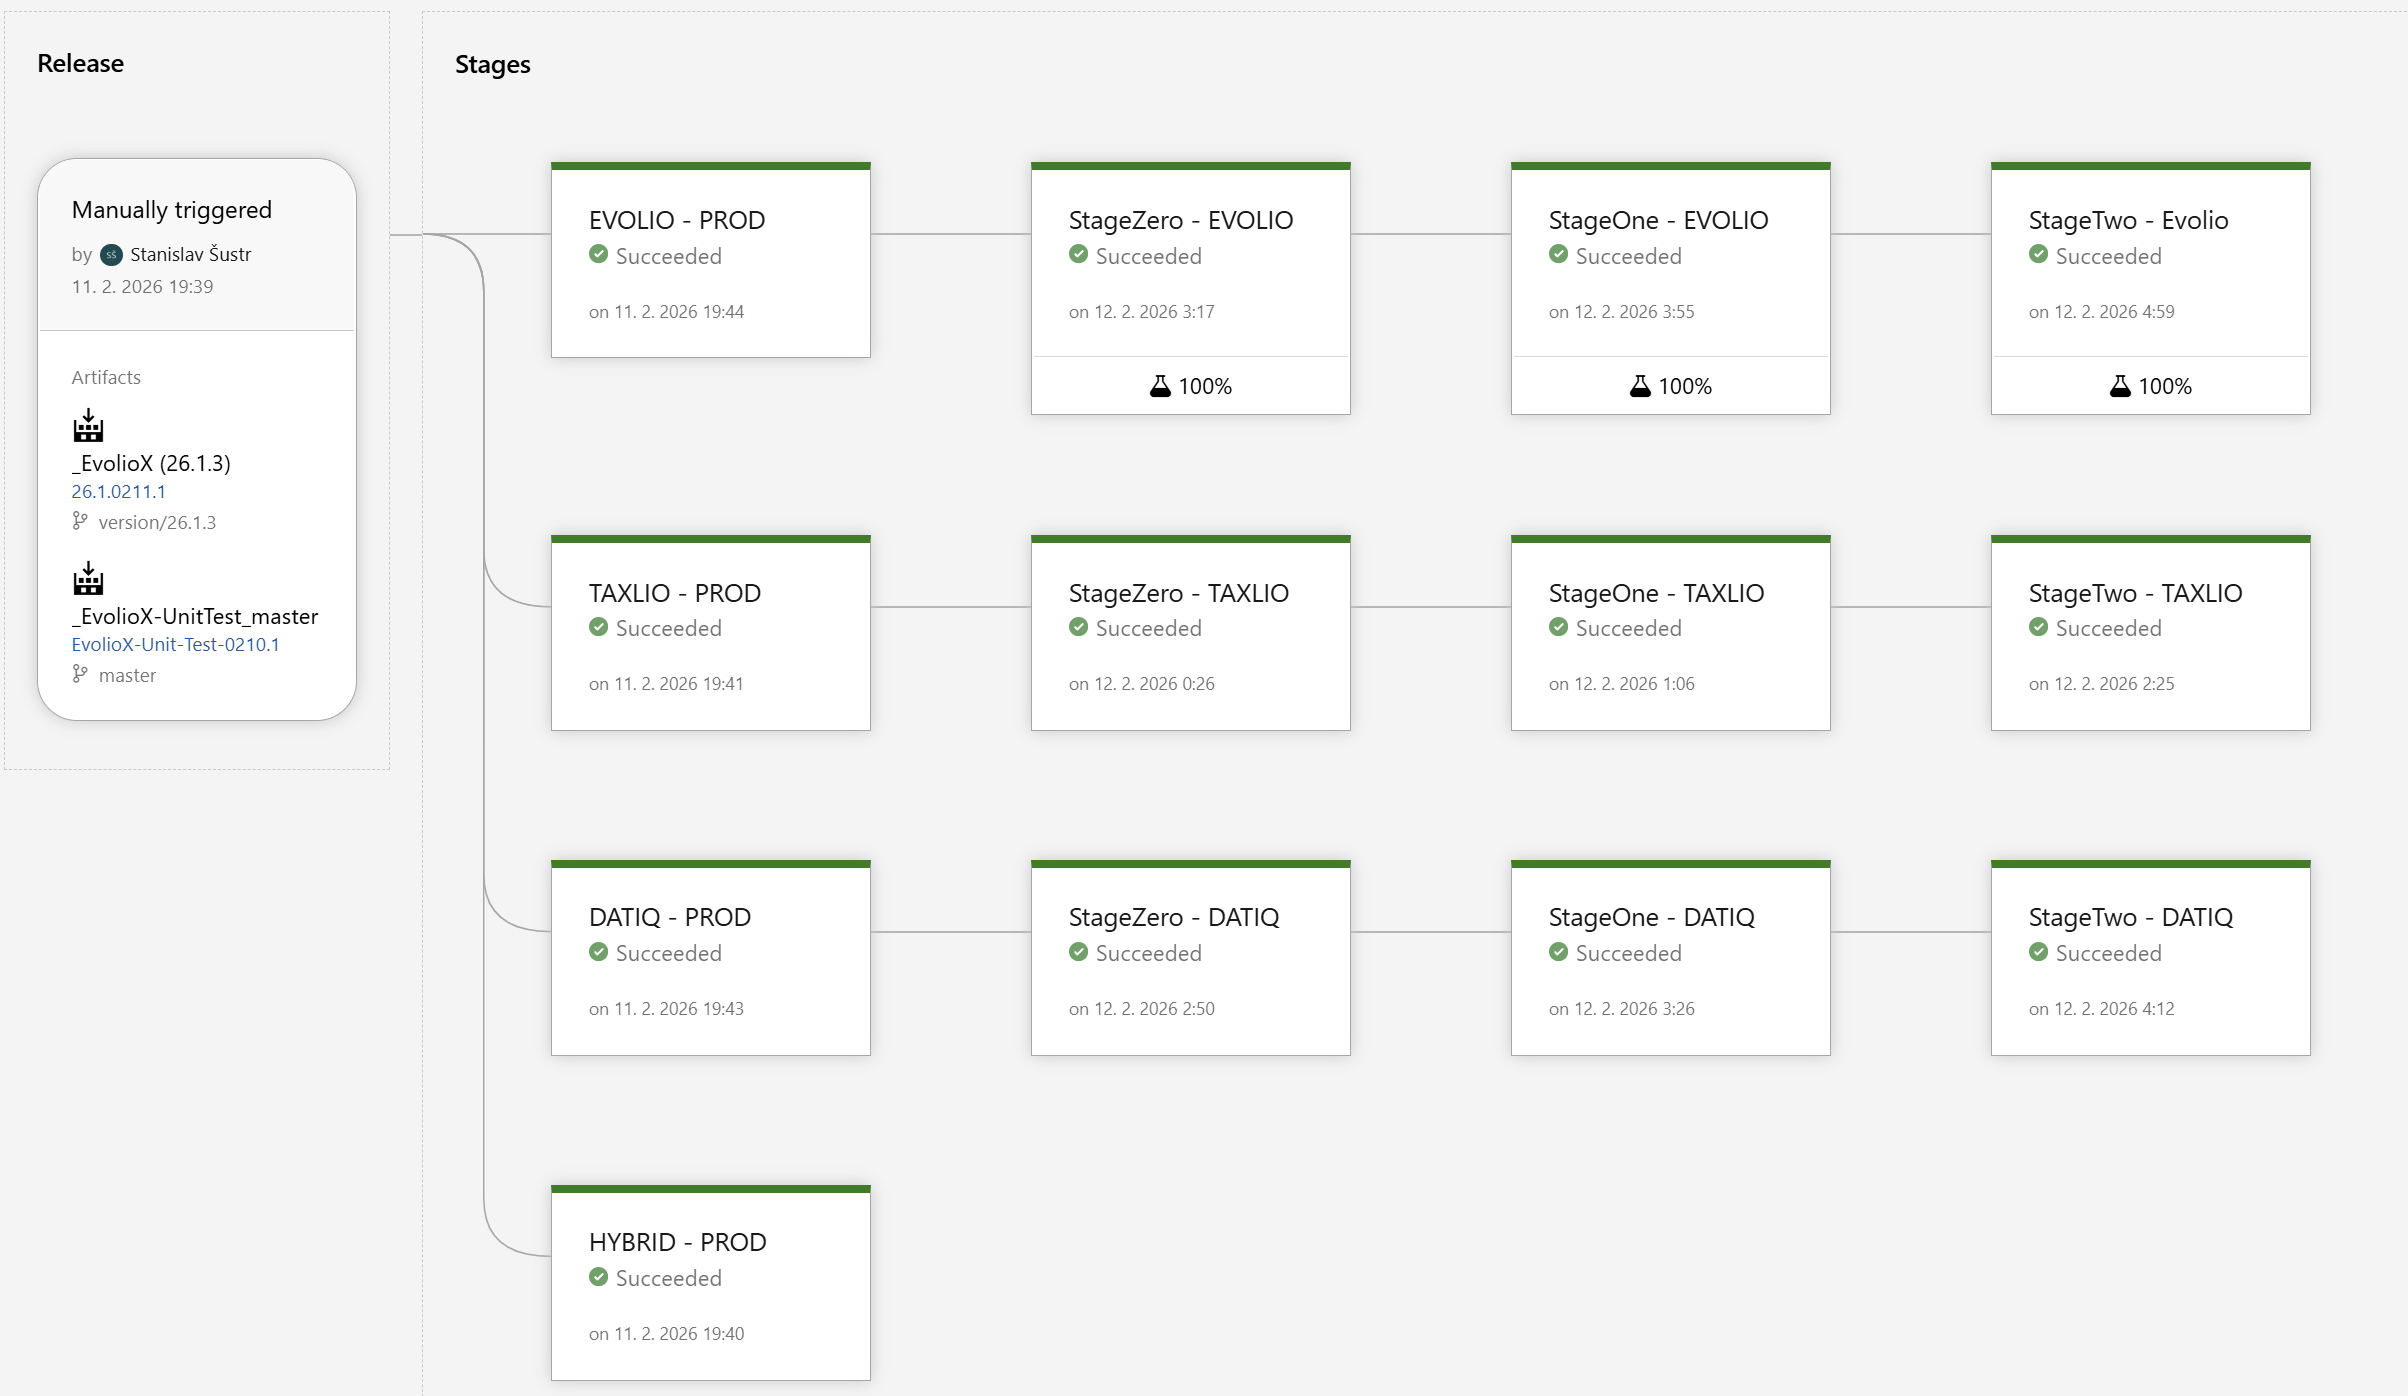
\includegraphics[width=1\textwidth]{Figures/DevOpsPipeline.png}
    \caption{Ukázka úspěšného běhu automatizovaných testů v release pipeline Azure DevOps}
    \label{fig:azure_devops}
\end{figure}

\subsection{Diagnostika chyb}
Pro efektivní řešení problémů je implementován mechanismus, který v případě pádu testu:
\begin{enumerate}
    \item Automaticky pořídí \textbf{screenshot} obrazovky v momentě chyby.
    \item Uloží systémové logy a stack trace.
    \item Tyto artefakty připojí k výsledku testu v Azure DevOps Dashboardu.
\end{enumerate}

Tato automatizace výrazně zrychluje proces debugování, protože umožňuje okamžitě identifikovat, zda chyba nastala v aplikaci (např. validační hláška) nebo v testu samotném.

\section{Přínos testovací sady}

Sada automatizovaných testů již v průběhu mé praxe opakovaně odhalila regresní chyby ještě před nasazením k zákazníkům -- konkrétní příklad je uveden v kapitole \ref{chap:evaluation}. Současný stav pokrývá klíčové CRUD operace hlavních agend (Podatelna, Případy, Subjekty, Fakturace) a jeho rozšíření o nové scénáře bylo jednou z mých průběžných činností. Pro další růst kvality by bylo vhodné doplnit nižší vrstvy pyramidy -- zejména integrační testy serverové logiky Add-inů, kde jsou dnes regrese odhalovány až UI testy, což je nákladnější z hlediska doby běhu a diagnostiky.

\chapter{Vazba praxe na studium}
\label{chap:studies_connection}

Odborná praxe mi umožnila konfrontovat teoretické znalosti získané studiem na Fakultě elektrotechniky a informatiky VŠB-TUO s reálnými požadavky softwarového vývoje. V mnoha oblastech jsem mohl přímo navázat na absolvované předměty, zatímco jiné domény vyžadovaly intenzivní samostudium.

\section{Uplatnění teoretických znalostí}

Nejvýznamnějším přínosem studia pro tuto praxi byla znalost objektově orientovaného programování a databázových systémů. Konkrétně jsem využil znalosti z následujících předmětů:

\begin{itemize}
    \item \textbf{Programování v C\# 1 a 2:} Znalost syntaxe jazyka C\#, typového systému a asynchronního programování byla nezbytná pro vývoj backendové části (Service Fabric Actor) a psaní automatizovaných testů.
    \item \textbf{Databázové systémy 1 a 2:} Při návrhu nových tabulek pro modul Importér a optimalizaci dotazů jsem uplatnil principy normalizace dat, tvorby indexů a práci s cizími klíči.
    \item \textbf{Funkcionální programování (FPR):} Ačkoliv je většina projektu psána v imperativních jazycích, principy rekurze probírané v tomto předmětu byly klíčové při implementaci hierarchického stromu kontextů (\textit{Context Tree}). Zobrazení vnořených struktur (např. Subjekt $\rightarrow$ Adresa $\rightarrow$ Kontakt) vyžadovalo rekurzivní průchod daty, což je koncept, který jsem si osvojil právě v FPR.
    \item \textbf{Správa softwarových projektů (SSP):} Základy verzování kódu pomocí systému Git, které byly představeny v tomto předmětu, jsem využíval denně při práci s větvemi (branches) a správě zdrojových kódů.
\end{itemize}
\chapter{Rozvoj kompetencí a chybějící znalosti}
\label{chap:competencies}

Přechod do firemního prostředí odhalil rozdíly mezi akademickými projekty a vývojem komerčního softwaru. Tato kapitola shrnuje technologie, které jsem se musel naučit samostudiem v průběhu praxe, a procesní aspekty, které ve výuce chyběly nebo byly pokryty jen povrchně.

\section{Nově osvojené technologie}

Největší výzvou byl vývoj moderního frontendu. Ačkoliv předmět \textit{Tvorba aplikací pro mobilní zařízení I} poskytuje základy jazyka JavaScript (Vanilla JS), pro práci na projektu Importér bylo nutné ovládnout komplexní ekosystém frameworku Angular a jazyka TypeScript.

\subsection{Reaktivní programování s RxJS}

Největším technologickým skokem bylo pochopení reaktivního programování. Koncept \texttt{Observable} — datového toku, na který se přihlásíme k odběru a reagujeme na příchozí hodnoty — byl zpočátku velmi odlišný od imperativního stylu, na který jsem byl zvyklý ze školních projektů.

V praxi jsem se nejčastěji setkával s operátory jako \texttt{forkJoin} pro paralelní volání více API najednou, \texttt{switchMap} pro zrušení předchozího požadavku při rychlém přepisování vstupu a \texttt{takeUntil} pro bezpečné odhlášení od odběru při zničení komponenty. Bez jejich pochopení by kód byl buď nefunkční, nebo by docházelo k tzv. memory leakům.

\subsection{Angular architektura}

Angular jako framework přináší přísnou strukturu, která zpočátku působí jako zbytečná komplexita, ale při vývoji rozsáhlejšího modulu se ukázala jako velká výhoda. Musel jsem pochopit systém Dependency Injection, který řídí, jak si komponenty a služby předávají závislosti, životní cyklus komponent (hooks jako \texttt{ngOnInit}, \texttt{ngOnDestroy}) a způsob, jakým Angular detekuje změny v datech a kdy překresluje UI.

Zvláštní pozornost si vyžádala strategie \textbf{OnPush}, kterou jsem musel nasadit u všech náročnějších komponent modulu Importér kvůli výkonu. Pochopení toho, kdy Angular komponentu překreslí a kdy ne, bylo klíčové pro odladění chyb, kde se UI neaktualizovalo po změně dat.

\subsection{Azure Service Fabric a architektura mikroslužeb}

Systém Evolio je postaven na platformě Azure Service Fabric, kde každá funkcionalita existuje jako samostatná služba (Actor nebo Service) s vlastním životním cyklem. Pro mě jako studenta zvyklého na monolitické aplikace bylo zpočátku obtížné pochopit, jak spolu tyto služby komunikují, jak se ladí chyba, která přechází přes hranice více služeb, a jak správně nastavit lokální vývojové prostředí tak, aby všechny závislosti fungovaly.

\section{Chybějící procesní znalosti}

Vedle technologií jsem si musel osvojit i řadu procesních dovedností, které jsou ve firemním prostředí samozřejmostí, ale ve školní výuce nejsou systematicky pokryty.

\subsection{Code Review a kultura zpětné vazby}

Každý kód, který jsem napsal, procházel před začleněním do hlavní větve revizí kolegy. Zpočátku bylo náročné přijímat připomínky k vlastnímu kódu a chápat je jako přirozenou součást procesu, nikoliv jako kritiku. Postupně jsem si ale zvykl na to, že code review odhaluje věci, které autor sám přehlédne, a naučil jsem se z komentářů kolegů aktivně čerpat znalosti o firemních konvencích a architektonických rozhodnutích.

\subsection{Práce v rozsáhlé sdílené kódové základně}

Na rozdíl od školních projektů, kde celý kód píše jeden člověk nebo malá skupina, systém Evolio tvoří stovky souborů vyvíjených souběžně více vývojáři. Naučil jsem se orientovat v cizím kódu, dohledávat kontext změn přes historii Gitu a dbát na to, aby moje změny nezasáhly do oblastí, na kterých paralelně pracuje kolega — čemuž slouží právě striktní větvení a pravidelné mergování.
\chapter{Zhodnocení výsledků a přínos praxe}
\label{chap:evaluation}

Cílem praxe bylo nejen zapojení do běžného chodu firmy, ale především dodání konkrétních softwarových řešení. Níže uvádím aktuální stav jednotlivých projektů.

\section{Modul Importér}
V době psaní této zprávy se nová webová verze Importéru nachází ve fázi \textbf{intenzivního testování}. Aplikace je plně funkční a probíhají konzultace s Team Leaderem a Product Ownerem ohledně doladění vizuálních detailů a user experience (UX).

Do testování jsou zapojeni také firemní konzultanti, kteří budou systém v budoucnu nejvíce využívat. Jejich zpětná vazba slouží k identifikaci posledních nedostatků před nasazením do ostrého provozu pro všechny klienty.

\section{AI Rozhraní}
Modul AI chatu pro specifického klienta byl úspěšně dokončen, nasazen do produkčního prostředí a je klientem aktivně využíván. Řešení splnilo požadavky na analýzu dokumentů a streamovanou komunikaci, přičemž klient vyjádřil s výsledkem spokojenost.

\section{Automatizované testy}
Sada automatizovaných testů byla integrována do CI/CD pipeliny a spouští se s každým vydáním nové verze. Testy již prokázaly svou reálnou hodnotu při odhalování regresních chyb.

Konkrétním příkladem úspěšného záchytu chyby byla situace, kdy testy odhalily nefunkčnost modálního okna pro editaci případu, pokud neobsahoval žádné subjekty. Chyba způsobovala "nekonečné načítání" a zablokování formuláře. Díky automatizaci byla tato kritická chyba zachycena ještě před nasazením k zákazníkům.

\chapter{Závěr}
\label{chap:conclusion}

Cílem mé odborné praxe ve společnosti AVE Soft s.r.o. bylo zapojení se do reálného vývojového procesu a realizace konkrétních softwarových úkolů v rámci systému Evolio. Hlavním výstupem byl návrh a implementace webového rozhraní pro modul Importér, který nahrazuje zastaralé desktopové řešení.

Během praxe se podařilo vytvořit moderní Single Page Aplikaci v technologii Angular, která komunikuje s nově vytvořeným backendovým doplňkem. Ačkoliv je modul momentálně ve fázi finalizace a testování, již nyní nabízí intuitivnější uživatelské rozhraní a zjednodušuje proces importu dat. Vedlejší úkoly, jako implementace AI chatu a tvorba automatizovaných testů, byly úspěšně dokončeny a nasazeny do provozu, kde přinášejí reálnou hodnotu jak firmě, tak jejím klientům.

Tato zkušenost pro mě byla klíčová pro pochopení fungování softwarové firmy. Osvojil jsem si moderní technologie, které nebyly součástí výuky (Angular, RxJS), a naučil se pracovat v týmu s využitím pokročilých nástrojů pro správu verzí a CI/CD. Praxe mi potvrdila, že kvalitní teoretický základ ze školy je nezbytný, ale pro uplatnění v oboru je nutné jej neustále rozvíjet samostudiem a reálnou prací na projektech.





%\input{Chapters/SampleChapter1.tex}
%\input{Chapters/SampleChapter2.tex}
%\input{Chapters/TechnicalDetails.tex}
%\input{Chapters/Conclusion.tex}

% Seznam literatury
\printbibliography[title={Literatura}, heading=bibintoc]

% Prilohy
\appendix
%\input{Chapters/Appendix1.tex}
%\input{Chapters/Appendix2.tex}

% Priloha vlozena primo do hlavniho LaTeX souboru. Ne vsechny prilohy je nutne mit ve zvlastnich souborech.
%\chapter{Dlouhý zdrojový kód}
%\lstinputlisting[label=src:CppExternal,caption={Dlouhý zdrojový kód v jazyce C++ načtený s externího souboru}]{SourceCodes/ArraySortingAlgorithms.cpp}

\end{document}
